\chapter{Background estimation}
\label{ch:bkgest}
\epigraph{\emph{The discipline of desire is the background of character.}}{John Locke}

	This chapter will describe the background estimation strategy for the main backgrounds of this analysis, already introduced in Section~\ref{sec:SMbkg}, and will give an overview of the systematic uncertainties - both experimental and theoretical - relevant for the analysis carried out. In particular, Section~\ref{sec:bkgest} provides an overview of the main reducible backgrounds and how they have been modelled in the analysis; in Section~\ref{sec:ddbkgest} the estimation of the irreducible background \ttZ\ will be extensively discussed, as it represents one of the author's major contribution to the analysis; finally, the systematic uncertainties will be presented in Section~\ref{sec:syst_unc}. The author also contributed to another analysis - the search for Dark Matter produced in association with third-generation quarks - through the estimation of the irreducible background \ttZ, which, again, was an irreducible background. The results of this analysis will be presented in Appendix~\ref{app:ttzdm}. 

	\section{Nominal background estimation}
	\label{sec:bkgest}

		\acp{CR} are implemented in order to estimate the various background yields in the \acp{SR}, so that one should not rely solely on the yields that one would obtain by applying the \ac{SR} selection to the \ac{MC} simulations of a background process. The \acp{CR} are designed to be selections orthogonal to the \acp{SR}. For example, one would ideally design a \ac{CR} such that it is fully dominated by a given background process, therefore suppressing the signal contamination. The \acp{CR} are used to derive a normalisation factor for each relevant background, by rescaling the expected \ac{MC} yields in the \ac{CR} to the observed number of data events in the same \ac{CR}. The prediction of the yields of a given background in \ac{SR} is then rescaled according to the normalisation found in the \ac{CR}. As an example, consider the case of one \ac{SR} and one \ac{CR}. Ideally, if the \ac{CR} is $100\%$ pure, the expected background yields in \ac{SR} $\left(N_{\mathrm{SR}}^{\mathrm{exp}}\right)$ can be written as:

		\begin{equation}
			N_{\mathrm{SR}}^{\mathrm{exp}} = \mu_{\mathrm{MC}} \cdot N_{\mathrm{SR}}^{\mathrm{MC}} \qquad \mathrm{with}\qquad \mu \equiv \frac{N_{\mathrm{CR}}^{\mathrm{data}}}{N_{\mathrm{CR}}^{\mathrm{MC}}} 
		\label{eq:exp_bkgyield}
		\end{equation}

		\noindent Here, $\mu$ is the normalisation scale factor, $N_{\mathrm{SR}}^{\mathrm{MC}}$ is the number of \ac{MC} events in \ac{SR}, $N_{\mathrm{CR}}^{\mathrm{MC}}$ is the number of \ac{MC} events in \ac{CR}, and $N_{\mathrm{CR}}^{\mathrm{data}}$ is the number of observed events in \ac{CR}. Furthermore, by defining the \ac{TF} as the ratio of the \ac{MC} yields in the \ac{SR} and \ac{CR}, one can define the expected background yields in the \ac{SR} as: 
		
		\begin{equation}
			N_{\mathrm{SR}}^{\mathrm{exp}} = T_f \cdot N_{\mathrm{CR}}^{\mathrm{data}} \qquad \mathrm{with} \qquad T_f \equiv \frac{N_{\mathrm{SR}}^{\mathrm{MC}}}{N_{\mathrm{CR}}^{\mathrm{MC}}}
		\label{eq:tf}
		\end{equation}

		\noindent This procedure allows a data-driven estimation of the expected background yields in the \ac{SR}, relying on the \ac{MC} simulation only for the computation of the \ac{TF}, and it is widely employed by several \ac{SUSY} analyses in \ac{ATLAS}. Furthermore, it also allows $N_{\mathrm{SR}}^{\mathrm{exp}}$ to be determined with an uncertainty given by the Poisson error on the $N_{\mathrm{CR}}^{\mathrm{data}}$ and the uncertainty on the \ac{CR}-to-\ac{SR} extrapolation. There are several background processes to be normalised in an independent set of \acp{CR}, and these usually have contamination from other background processes. The above-mentioned equations then turn into a system of $n$ equations (Equation~\ref{eq:mu_factors}), with $n$ number of background processes to control. These are then solved to obtain the various normalisation factors ($\mu_i$):

		\begin{equation}
			\begin{cases}
				N_{\mathrm{CR,1}}^{\mathrm{data}} = \mu_1 N_{\mathrm{CR,1}}^{\mathrm{MC,1}} + \mu_2 N_{\mathrm{CR,1}}^{\mathrm{MC,2}} + \dots + \mu_n N_{\mathrm{CR,1}}^{\mathrm{MC,n}} \\
				N_{\mathrm{CR,2}}^{\mathrm{data}} = \mu_1 N_{\mathrm{CR,2}}^{\mathrm{MC,1}} + \mu_2 N_{\mathrm{CR,2}}^{\mathrm{MC,2}} + \dots + \mu_n N_{\mathrm{CR,2}}^{\mathrm{MC,n}} \\
				\dots \\
				N_{\mathrm{CR,n}}^{\mathrm{data}} = \mu_1 N_{\mathrm{CR,n}}^{\mathrm{MC,1}} + \mu_2 N_{\mathrm{CR,n}}^{\mathrm{MC,2}} + \dots + \mu_n N_{\mathrm{CR,n}}^{\mathrm{MC,n}} \\
			\end{cases}
		\label{eq:mu_factors}
		\end{equation}

		\noindent Here, $N_{\mathrm{CR,j}}^{\mathrm{MC,i}}$ is the number of events in the $i^{\mathrm{th}}$ process, taken from the \ac{MC} simulation, that passed the $j^{\mathrm{th}}$ CR selection, and $N_{\mathrm{CR,k}}^{\mathrm{data}}$ is the number of data events in the observed $k^{\mathrm{th}}$ \ac{CR}. Such procedure is validated in so-called \acp{VR}, designed to be ``in between'' \acp{CR} and \acp{SR}. The purpose of the \acp{VR} is to validate the background estimation in the \acp{CR} in a region close to the \acp{SR}, so that when extrapolating the background estimation from \ac{CR} to \ac{SR} there is no bias in the estimated \acp{TF}. A sketch of how \acp{SR}, \acp{CR}, and \acp{VR} are selected is shown in Figure~\ref{fig:extrapolation}. If the estimate in the \ac{CR} is correct, the background expected in the corresponding \ac{VR} should match the number of observed data events in the \ac{VR}. The data-\ac{MC} agreement in \acp{VR} represents a green light towards the unblinding of the blinded \acp{SR}.

		\begin{figure}[!htb]
		  \begin{center}
		   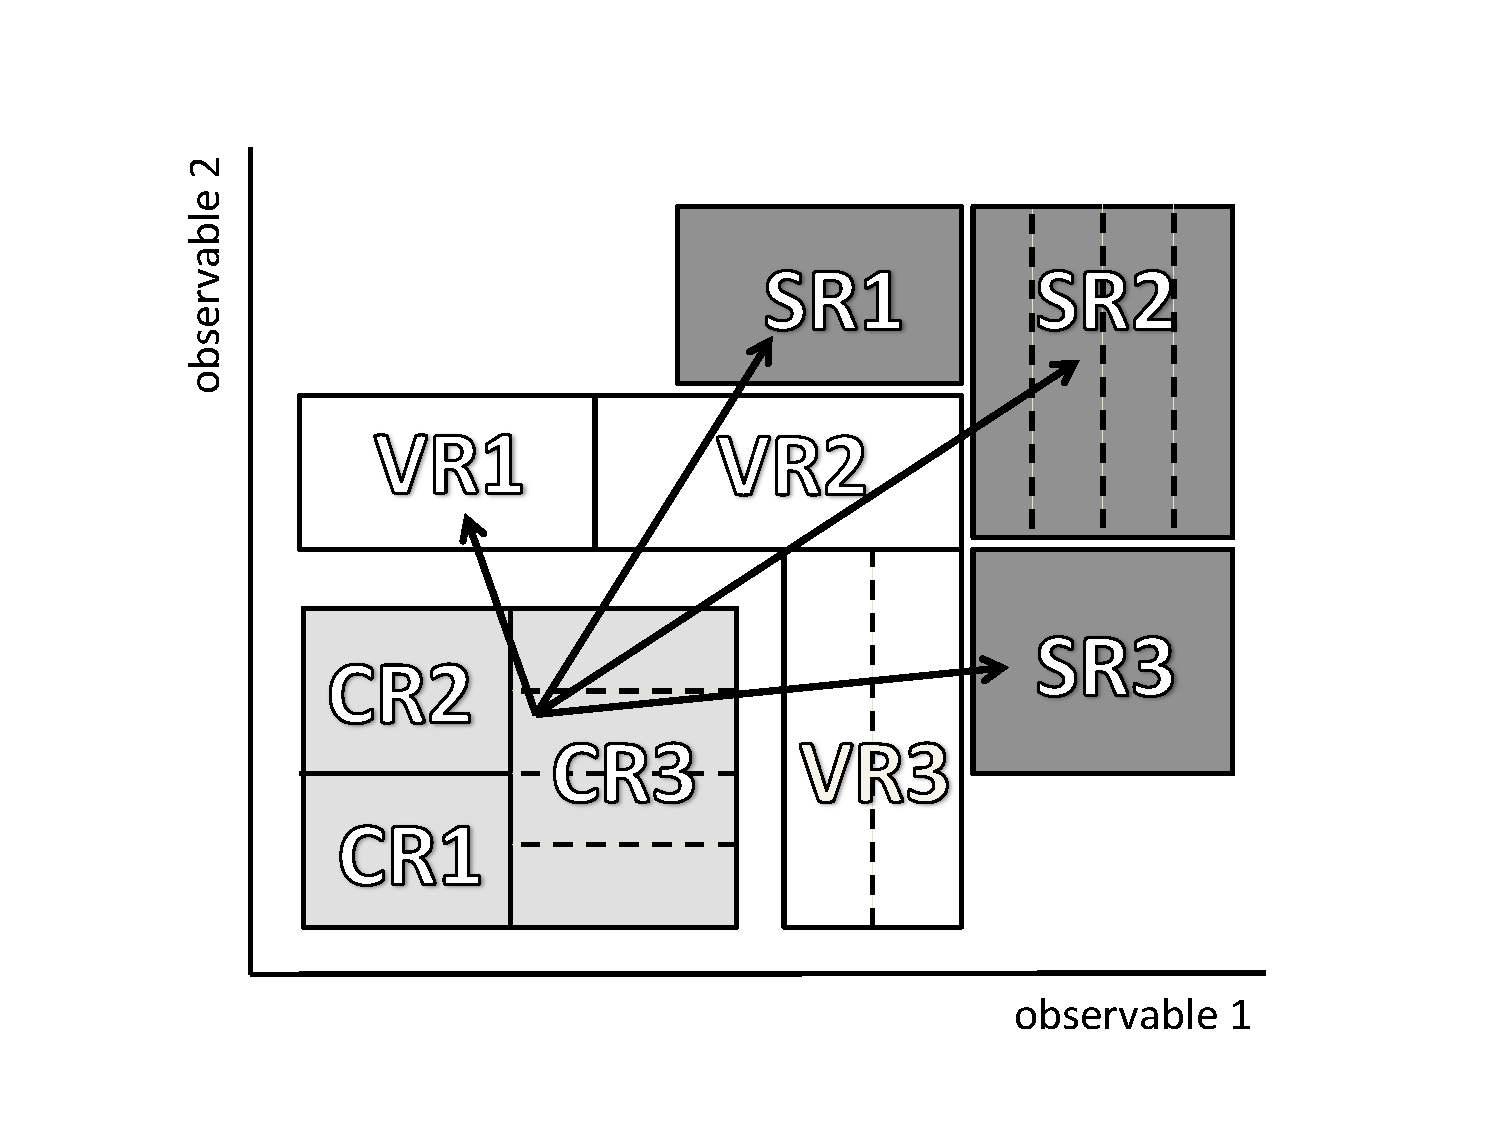
\includegraphics[width=\textwidth]{figures/stop/cartoon_CRVRSR_bw}
		   \caption{A schematic view of an analysis strategy with multiple \acp{CR}, \acp{VR}, and \acp{SR} using two observables. The \ac{CR}-to-\ac{SR} extrapolation is verified by employing \acp{VR} that lie in the extrapolation phase space (taken from~\cite{histfitter}.}
		   \label{fig:extrapolation}
		  \end{center}
		\end{figure}

		For the estimation of the major sources of reducible background, $1$-lepton and $2$-lepton \acp{CR} are employed. In particular, a $2$-lepton \ac{CR} is used for the estimation of the \Zjets\ background (CRZ) and a $1$-lepton \ac{CR} is employed for the estimation of \ttbar\ (CRT), single top (CRST), and \Wjets\ (CRW) backgrounds. Additionally, a dedicated set of variable is employed:

		\begin{description}
			\item[\boldmath $N_{\ell}$:] number of leptons in the event;
			\item[\boldmath $\pt^{\ell}$:] transverse momentum of the leading lepton;
			\item[\boldmath $m_{\ell\ell}$:] invariant mass of the \ac{SFOS} lepton pair in the event;
			\item[\boldmath $\mT(\ell,\met)$:] transverse mass calculated from the \met\ and the transverse momentum of the lepton;  
			\item[\boldmath $\metprime$:] the transverse momenta of the selected leptons are added to the \ptmiss, \eg\ to mimic the \Znunu\ decays in the \acp{SR}, forming the quantity \metprime. Essentially, this is a corrected version of \met\ to treat the leptons as neutrinos. The \emph{prime} notation is used for all the variables that depend on \metprime.
		\end{description}


		\subsection{Control regions definition}
		\label{subsec:crs}

			The background estimation strategy is based on five independent \acp{CR} to control \Zjets, \ttbar, single top, \Wjets, and \ttZ\ backgrounds. Where enough statistics are available, \acp{CR} are designed to estimate backgrounds in different kinematic regions of the \acp{SR}. A description of the nominal background estimation strategy is given below, except for the estimation of the irreducible background \ttZ, which will be discussed in Section~\ref{sec:ddbkgest} as a different technique is employed. The remaining backgrounds whose contributions are negligible are di-bosons and multi-jet. The former is estimated directly using the yields obtained from \ac{MC} simulations. The latter is estimated using the \emph{jet smearing} method, a procedure described in~\cite{Aad:2012fqa} and~\cite{calumThesis} which will not be discussed. A detailed description of all the selections employed for the estimation of the above-mentioned backgrounds can be found in Appendix~\ref{app:sumbkgest}. 

			\begin{description}
			%\paragraph{$2$-lepton \Zjets\ CR}

				\item [\Zjets\ CR (CRZ)] The estimation of the \Znunu\ background is performed via the design of a $2$-lepton $Z \rightarrow \ell \ell$ \ac{CR}. Although the branching fraction of \Zll\ is smaller than \Znunu, a purer \ac{CR} can be obtained by defining the \ac{CR} in such a way. As all the \acp{SR} (exception made for SRD) have requirements on the \MET\ selection, jet multiplicity, and $b-$tagged jets, in order to ensure as little \ac{CR}-to-\ac{SR} extrapolation as possible the same kinematic cuts are applied in CRZ. SRA and SRB share a set of two \Zboson\ \acp{CR}: one is shared by the TT and TW categories (due to statistical limitations) and one is dedicated to the T0 category (CRZAB-TT-TW, CRZAB-T0). A common \Zboson\ \ac{CR} is used for SRD (CRZD). Finally, a \Zboson\ \ac{CR} with tighter \HT\ requirements is used for SRE. The \acp{CR} are defined by using events passing a single-lepton trigger, and in addition requiring a cut on $2$ \acl{SFOS} leptons. To reduce the top contamination, the requirements $\met < 50$ \GeV, and  $\metprime > 100$ \GeV\ are applied. Furthermore, a $\Zboson$-mass window cut on the invariant mass of the leptons pair is applied, to reduce other backgrounds contamination. A detailed \ac{CR} definition is given in Table~\ref{tab:selectionCRZs}

			%\paragraph{$1$-lepton CR for \ttbar, single top, and \Wjets}
		
				\item [\ttbar\ CR (CRT)] As already mentioned, these \acp{CR} are all defined by using events required to pass a \met\ trigger. In addition, in order to emulate the hadronic $\tau$ decays in the \acp{SR} the lepton is treated as a non-$b$-tagged jet in the computation of all jet-related variables. Similarly to CRZ, CRT is then further divided to address the various \acp{SR} (see Table~\ref{tab:selectionCRTs}).

				\item [\Wjets\ CR (CRW)] CRW, very similar to CRT, also employs a \met\ trigger, but here only $1$ \bj\ is required. In addition, a looser and inverted cut on \mantikttwelvezero, together with a requirement $\Delta R(b_{0,1},\ell)_{\mathrm{min}}$, defined as the minimum $\Delta R$ between the two jets with the highest $b$-tag weight and the selected lepton, ensures that CRW is orthogonal to CRT (see Table~\ref{tab:selectionCRWST}). 

				\item [Single top CR (CRST)] In CRST, also similar to CRT and CRW, two \bjs\ are required. Furthermore, the requirement on the $\Delta R$ of the two leading-weight \bjs\ is necessary to reject a large part of the remaining \ttbar\ background (see Table~\ref{tab:selectionCRWST}).
			\end{description}

			%Ultimately, Tables~\ref{tab:selectionCRTs} and~\ref{tab:selectionCRWST} provide the detailed definitions of the CRT, and CRST and CRW, respectively.


		\subsection{Validation regions}

			To validate the estimation of the various backgrounds, \acp{VR} are employed where possible. In particular, the following \acp{VR} are defined:

			\begin{description}

				\item [\Zjets\ VR (VRZ)] $0$-lepton \acp{VR} are designed to validate the background estimate for \Zjets\ in the \acp{SR}. Similarly to the strategy used in the \ac{CR}, dedicated sets of \acp{VR} are employed: VRZAB, VRZD, VRZE. No VRZ is designed for SRC due to the negligible contribution of the \Zboson\ background in this region. In practice, to ensure orthogonality to the \acp{SR}, the requirement on one or more of the following variables is inverted: \drbjetbjet, \mantikttwelvezero, \mantikteightzero. A detailed list of the VRZ selections, after the common pre-selection shown in Table~\ref{tab:SRcommon}, is shown in Table~\ref{tab:selectionVRZs}.

				\item [\ttbar\ VR (VRTT)] Following the same strategy discussed so far, in order to validate the \ttbar\ background, $0$-lepton \acp{VR} sharing the same common pre-selection close to the SRA and SRB definitions are designed for each of the top categories: VRTA-TT, VRTA-TW, VRTA-T0, VRTB-TT, VRTB-TW, VRTB-T0. To ensure orthogonality with the \acp{SR} the \mtbmin\ requirement is inverted in all \acp{VR}. In particular, for the definition of VRTA, the SRA requirements are unchanged except for \mttwo\, which is not being applied, $100<\mtbmin<200\gev$, and the \met\ requirement being loosened by $100$ \GeV. The requirements for VRTB are the same as in the \acp{SR} except for \mtbmin, being changed to $100<\mtbmin<200\gev$ for VRTB-TT, $140<\mtbmin<200\gev$ for VRTB-TW, and $160<\mtbmin<200\gev$ for VRTB-T0. The VRTC keeps the same requirements as \SRC\ except for the looser requirements of $\mS> 100\gev$, $\pTSFour>40\gev$ and $\nJetS > 4$. The \dPhiISRMET\ requirement is inverted and $\mV/\mS<0.6$ is applied in addition to the existing selection. The \ac{VR} VRTD, targeting SRD, is formed by applying the following requirements: $100<\mtbmin<200\gev$, $\ptbzero+\ptbone>300\gev$, $\ptthree>80$ \GeV, and $\mtbmax>300$ \GeV. All other requirements are applied exactly as in SRD-low except for the requirement on \ptfour\ which is not applied. Finally, VRTE, dedicated to SRE, ensures a minimum extrapolation as it applies the same requirements on the number of $b$-jets, \mantikteightzero, and \mantikteightone, and inverts the \mtbmin\ requirement to $100<\mtbmin<200\gev$ (see Tables~\ref{tab:VRTABDef} and~\ref{tab:VRTCDEDef}).

				\item [\Wjets\ VR (VRW)] For the validation of the \Wjets\ background a unique $1$-lepton-$1$-\bj\ \ac{VR} is used to test such background in all the \acp{SR}, with the only difference with respect to CRW being \mindrblep, which is greater than $1.8$ in the \ac{VR} plus two additional requirements, namely $\mtbmin>150$ GeV and $\mantikttwelvezero<70$ \GeV\ which are included in the definition of VRW (see Table~\ref{tab:VRW}).

			\end{description}

		Ultimately, in order to determine the normalisations of the \ac{SM} backgrounds for \Zboson, \ttbar, \Wboson, single top, \ttZ, and their estimates, in each \acp{SR}, the observed numbers of events in the various \acp{CR} are included in a binned profile likelihood fit, which will be discussed in Section~\ref{sec:stat_ana}. A simultaneous fit, to best match the observed data in each \ac{CR}, taking into account all the contributions from the various backgrounds, is performed to determine the \ac{SM} background normalisation factors. 


	\section{Estimation of the \protect{\ttZ} irreducible background}
	\label{sec:ddbkgest}

		The production of top pairs in association with a vector boson (\ttV) is the second most important background in most \acp{SR}. Precisely, such background is completely dominated by $\ttZ(\to \nu\bar{\nu})$, as the $\ttW(\to \ell \nu)$ contribution in the \ac{SR} is negligible due to the presence of the lepton in the final state. As already anticipated in various parts of this work, $\ttZ(\to \nu\bar{\nu})$ yields a final state with kinematic properties identical to the signal, namely two top quarks (six jets, if both tops are fully reconstructed) and \met\ from the neutrinos coming from the \Zboson\ decay. Unfortunately, as of today, although the \ac{ATLAS} collaboration has allocated some effort on this, no \ac{SM} measurement of such process has been published, especially due to the presence of large \met\ making the isolation of such signature quite difficult.

		%The analysis carried out during Run-1~\cite{stop0LRun1} did not employ any \ac{CR} for such background, relying the estimation of its contribution in \ac{SR} solely on the yields obtained from the \ac{MC} simulation. For the analysis presented in this work, one attempt to isolate such background was made using a $3$-lepton $\ttZ(\to\ell\ell)$ \ac{CR}, one lepton from the semi-leptonic \ttbar\ decay and $2$ leptons from the leptonic decay of the \Zboson, although due to the large extrapolation on the number of leptons and the low statistics (low branching fraction to leptons), the design of a $3$-lepton \ac{CR} was dropped. Furthermore, a $2$-lepton \ac{CR} would suffer a large contamination from \ttbar\ and \Zjets\ backgrounds, therefore both methods were dropped and will not be further discussed.

		A data-driven technique, similar to the one adopted in~\cite{stop1L}, is employed to estimate this background. The normalisation of \ttZ\ in the \ac{SR} is estimated by designing a $1$-lepton-$1$-photon \ttgamma\ control region (CRTTGamma). Despite the difference in cross-section ($\sigma_{\ttZ}^{\mathrm{aMC@NLO}} \sim 150$ pb, $\sigma_{\ttgamma}^{\mathrm{aMC@NLO}} \sim 215$ pb), the validity of the technique is supported by the similarities of the \ttZ\ and \ttgamma\ Feynman diagrams, as shown in Figure~\ref{fig:ttZttGamma}. This \ac{CR} is designed to minimise the differences between the two processes and keep the theoretical uncertainties from the extrapolation of the $\gamma$ to the \Zboson\ as small as possible. 

		\begin{figure}[htpb]
		  \centering
		  	\subbottom[]{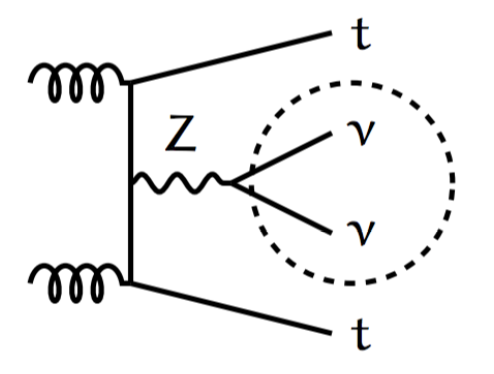
\includegraphics[width=0.48\textwidth]{figures/stop/ttZ}}
			\subbottom[]{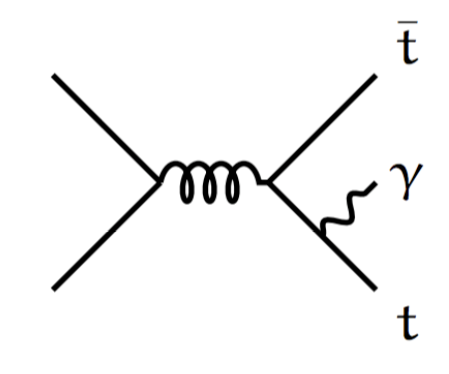
\includegraphics[width=0.48\textwidth]{figures/stop/ttGamma}}
		    \caption{Diagrams of the production of top-antitop pairs associated with a \Zboson\ boson~(a) and a photon~(b).}
		    \label{fig:ttZttGamma}
		\end{figure}

		The strategy is based on the addition of the transverse momentum of the $\gamma$ in the event $\left(\pt^{\gamma}\right)$ to the computation of the \met\ to mimic the neutrinos from the \Zboson\ decay. In this context, the $\gamma$ \pt\ is approximately the missing transverse momentum, $\pt^{\gamma} \sim \met$. 

		Events in this \ac{CR} are required to pass the same lepton triggers and lepton-\pt\ requirements required in all the other $1$-lepton \acp{CR}. In addition, an isolated photon with $\pt^{\gamma} > 150$ \GeV\ is required. Figure~\ref{fig:ZGammaratio} shows the truth-level \pt\ distributions of the \Zboson\ and the $\gamma$. The former is taken from the \ttZ\ \ac{MC} sample and obtained by requiring a basic \ac{SR}-like selection comprising at least four jets, two of which $b$-tagged, zero baseline and signal leptons, and a lower cut of $150$ \GeV\ on the \pt\ of the \Zboson. The latter is taken from the \ttgamma\ \ac{MC} sample and obtained by requiring a basic \ac{CR}-like selection including at least four jets, two of which $b$-tagged, $1$ lepton and $1$ photon, and a lower cut of $150$ \GeV\ on the \pt\ of the $\gamma$. The agreement found in Figure~\ref{fig:ZGammaratio} ensures the applicability of the method and, more importantly, that the shape of the \pt\ distributions of the two bosons taken from the two \ac{MC} samples, is essentially the same in the whole kinematic range. This, in turn, ensures that the extrapolation of the \ttZ\ yields in \ac{SR} from the CR $\left(\pt^{\gamma}\right)$ to SR $\left(\met\right)$ will be safe. In addition, similarly to what is done for CRZ, the photon \pt\ is used for the estimation of \met-related variables. Finally, in order to avoid double-counting of \ttbar\ simulated events where a hard photon is emitted, the \verb+MCTruthClassifier+~\cite{MCTruthClassifier} tool is employed to perform a truth-level selection of photons irradiated by a top quark. Table~\ref{tab:CRTTGamma} shows the detailed selection applied. 

		\begin{figure}[htpb]
		  \centering
		  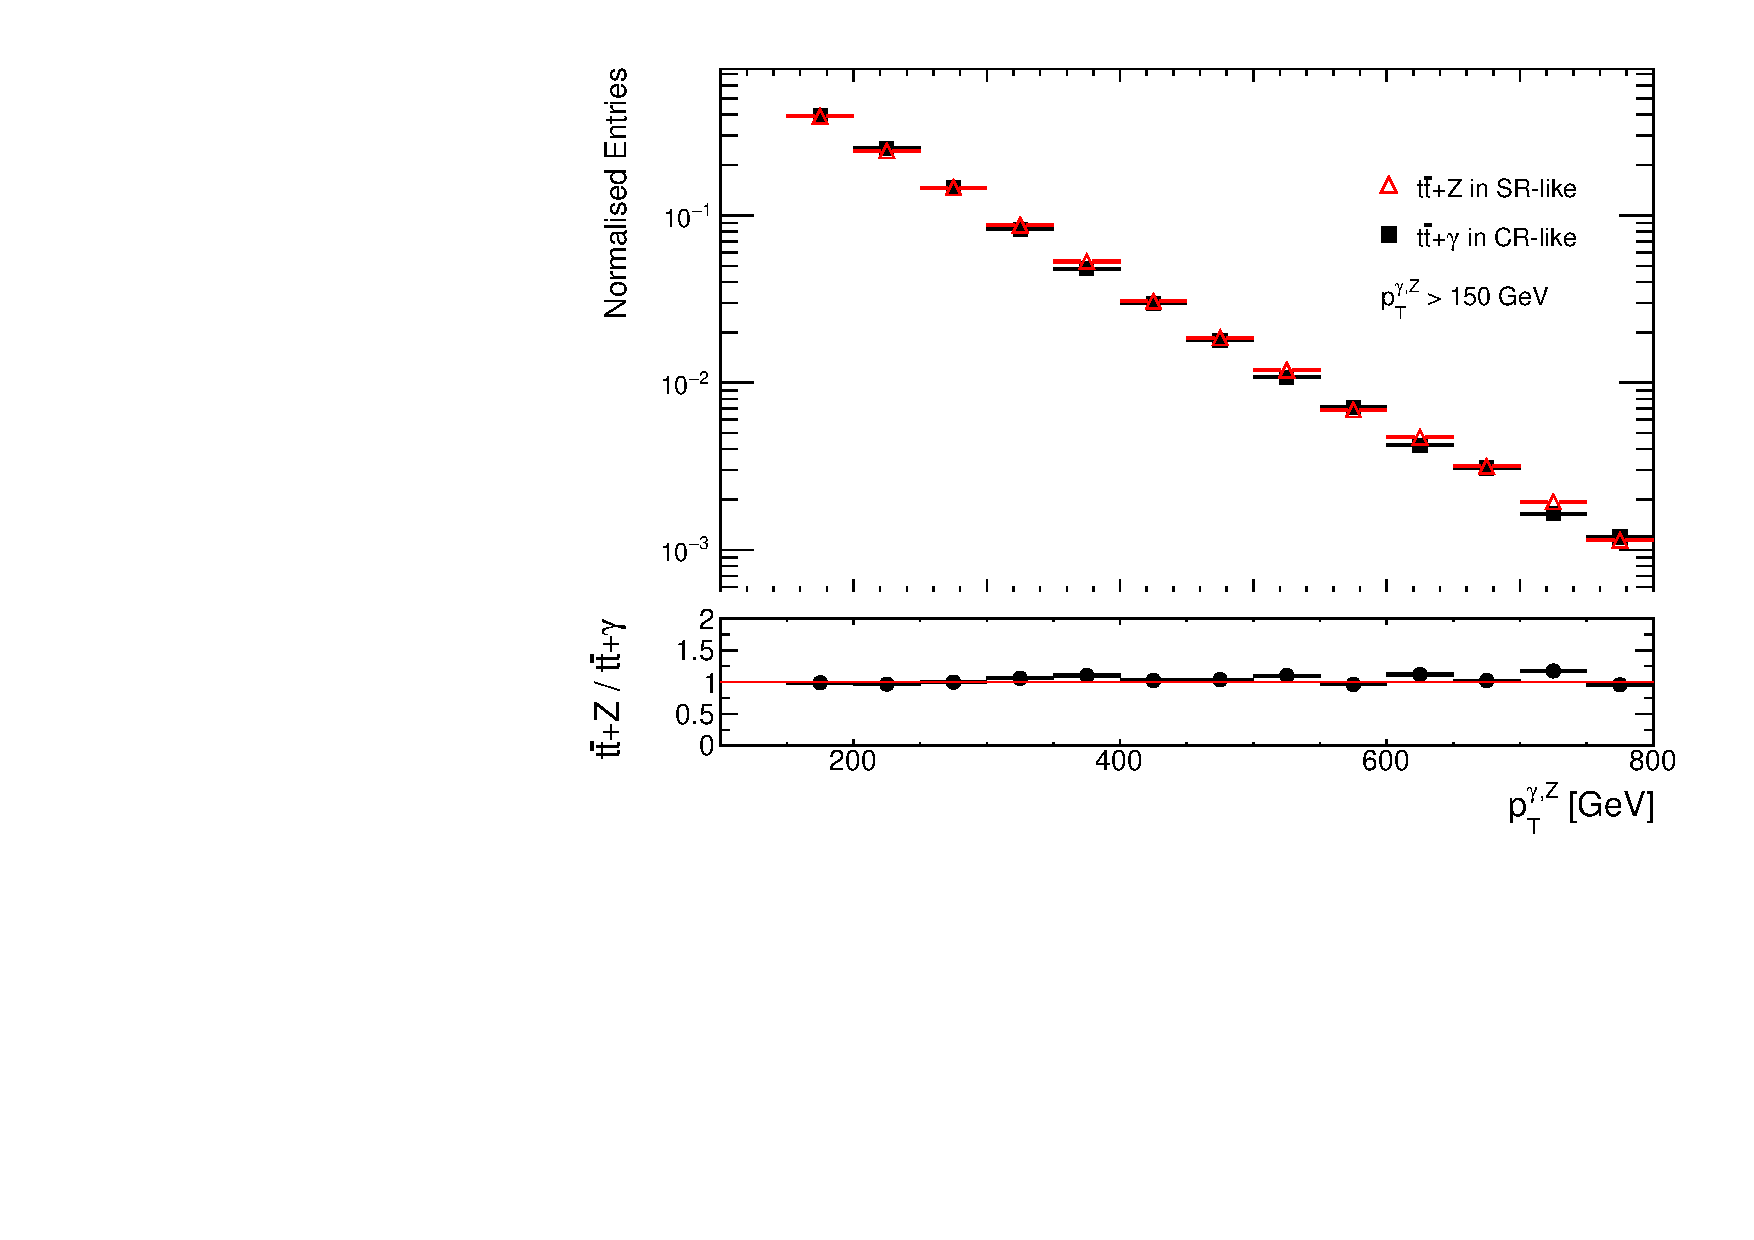
\includegraphics[width=\textwidth]{stop/ttg-int-nonpub/TruthStudies/ZGammaRatio.pdf}
		  \caption{Ratio plot of the \pt\ of the \Zboson\ and $\gamma$ bosons at truth level obtained by requiring \ac{CR}-like and \ac{SR}-like selections as described in the text.}
		  \label{fig:ZGammaratio}
		\end{figure}

		The estimation of the \ttZ\ yields in the \ac{SR} is based on an approximation of what was already shown in Equations~\ref{eq:tf} and~\ref{eq:mu_factors}:
		
		\begin{equation}
			N_{\ttZ,\mathrm{SR}}^{\mathrm{exp}} \sim N_{\mathrm{CR}}^{\mathrm{obs}} \cdot \frac{N_{\ttZ,\mathrm{SR}}^{\mathrm{MC}}}{N_{\ttgamma,\mathrm{CR}}^{\mathrm{MC}}} \qquad \mathrm{with} \qquad T_f \equiv \frac{N_{\ttZ,\mathrm{SR}}^{\mathrm{MC}}}{N_{\ttgamma,\mathrm{CR}}^{\mathrm{MC}}}
		\label{eq:ttZ_estimation}
		\end{equation}

		\noindent where, $N_{\ttZ,\mathrm{SR}}^{\mathrm{exp}}$ is the expected \ttZ\ yields in the \ac{SR}, $N_{\mathrm{CR}}^{\mathrm{obs}}$ is the observed number of events in the \ttgamma\ \ac{CR}, $N_{\ttZ,\mathrm{SR}}^{\mathrm{MC}}$ is the number of \ttZ\ events falling into the \acp{SR}, and $N_{\ttgamma,\mathrm{CR}}^{\mathrm{MC}}$ is the number of \ttgamma\ events in the \ttgamma\ \ac{CR} taken from the \ac{MC} simulation. As previously mentioned, if the \ac{CR} were $100\%$ pure (no contamination from other background processes) Equation~\ref{eq:ttZ_estimation} would not be approximate, but exact.

		\begin{table}
			\parbox{.45\linewidth}{
			\centering
			\captionof{table}{Selection criteria for CRTTGamma.}\label{tab:CRTTGamma}
		   	\begin{tabular}{lc}
			      \toprule
			      \textbf{Selection}  & \textbf{CRTTGamma} \\
			      \toprule
			      Trigger & lepton \\ 
			      $N_{\ell}$ & 1 \\
			      Lepton \pt & $28$ GeV \\
			      \midrule
			      $N_{\gamma}$ & $1$\\
			      $\gamma$ \pT\ & $> 150$ \GeV \\
			      \midrule
			      $N_{\mathrm{jets}}$ & $ \geq 4 $ \\
			      Jet \pT\ & $(80,80,40,40)$ \GeV \\
			      $N_{\bjs}$ & $\ge 2$ \\
			      \bottomrule
			   \end{tabular}
			}
			\hfill
			\parbox{.45\linewidth}{
			\centering
			\captionof{table}{Background composition of \ttgamma\ \ac{CR}. The yields are obtained pre-fit. The uncertainties shown are statistical only.}% $\mu_{\ttgamma}$ is the background normalisation factor obtained from the fit that will be discussed in Section~\ref{sec:stat_ana}.}
			\label{tab:CRTTGamma_yields}
				\begin{tabular}{lc}
					\toprule
					\textbf{Process} & \textbf{Yield} \\
					\toprule
					\ttgamma & $111.76 \pm 1.45$ \\
					$V+\gamma$ & $6.29 \pm 0.63$ \\
					$\ttbar$ & $5.14 \pm 1.20$ \\
					$\ttV$ & $2.34 \pm 0.25$ \\
					single Top & $2.07 \pm 0.80$ \\
					$Z$ & $0.66 \pm 0.17$ \\
					$W$ & $0.04 \pm 0.02$ \\
					\midrule
					Total MC & $128.29 \pm 2.17$ \\
					Data & $161$ \\
					\midrule
					\multicolumn{2}{c}{\textbf{CRTTGamma} ( $87\%$)} \\ 
					\midrule
					$\mu_{\ttgamma}$ & $1.29 \pm 0.12$ \\
					\bottomrule
				\end{tabular}
			}
		\end{table}

		Table~\ref{tab:CRTTGamma_yields} shows the breakdown of the various processes entering into the CRTTGamma selection shown in Table~\ref{tab:CRTTGamma}. The purity, defined as the number of simulated \ttgamma\ events divided by the total number of simulated events, is $87\%$. The normalisation factor, $\mu_{\ttgamma} = 1.29$, defined in Equation~\ref{eq:mu_ttgamma} (where $N_{\mathrm{TOT,CR}}^{\mathrm{MC}}$ represents the total number of simulated events falling into the \ttgamma\ \ac{CR}), is obtained. 

		\begin{equation}
			\mu_{\ttgamma} = \frac{ N_{\mathrm{CR}}^{\mathrm{obs}} - \left ( N_{\mathrm{TOT,CR}}^{\mathrm{MC}} - N_{\ttgamma, \mathrm{CR}}^{\mathrm{MC}} \right ) } { N_{\ttgamma,\mathrm{CR}}^{\mathrm{MC}} }
			\label{eq:mu_ttgamma}
		\end{equation}

		Additionally the agreement between the observed data and the \ac{MC} predictions was checked in the \met\ and \mtlepmet\ distributions, shown in Figure~\ref{fig:fakes_check}, to rule out any potential fake lepton that would show up at low values of \mtlepmet. The agreement found in the low \mtlepmet\ region is a reasonable indication of no significant fake contributions.

		\begin{figure}[htbp]
			\begin{center}
				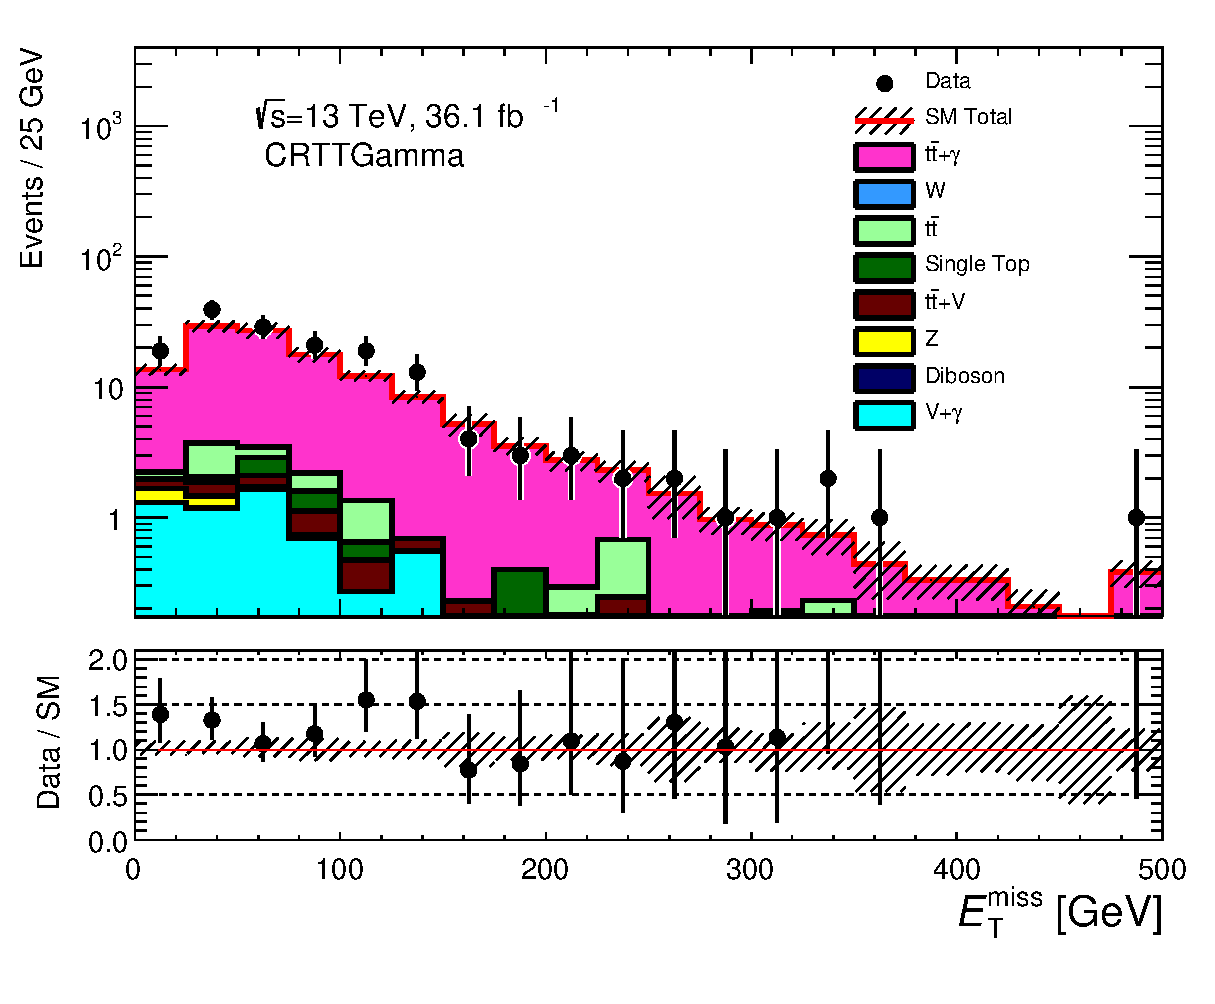
\includegraphics[width=0.49\textwidth]{figures/stop/ttg-int-nonpub/Met_CRTTGamma_withRatio_log}
				%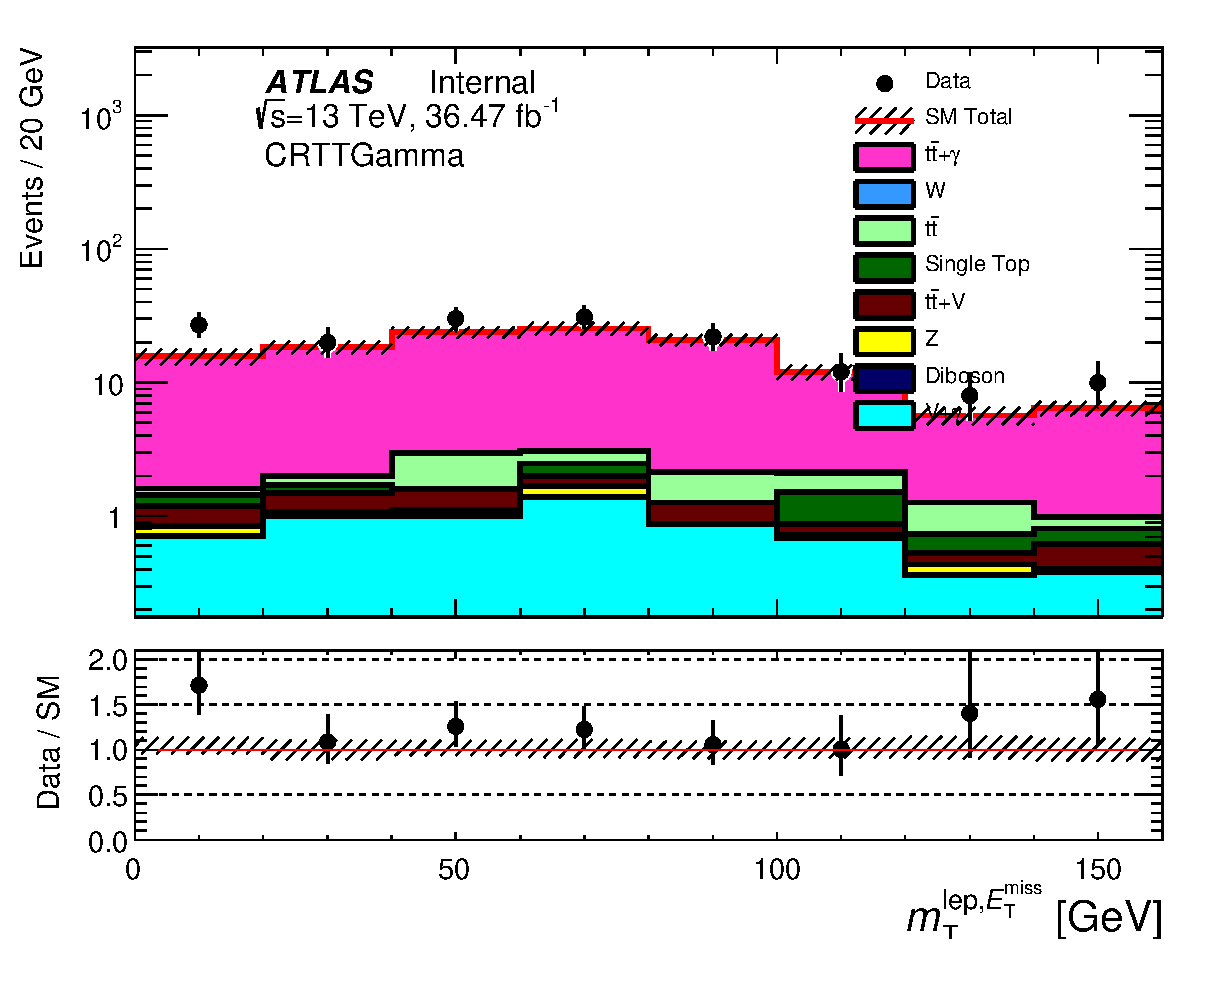
\includegraphics[width=0.49\textwidth]{figures/stop/ttg-int-nonpub/MtMetLep_CRTTGamma_withRatio_log}
				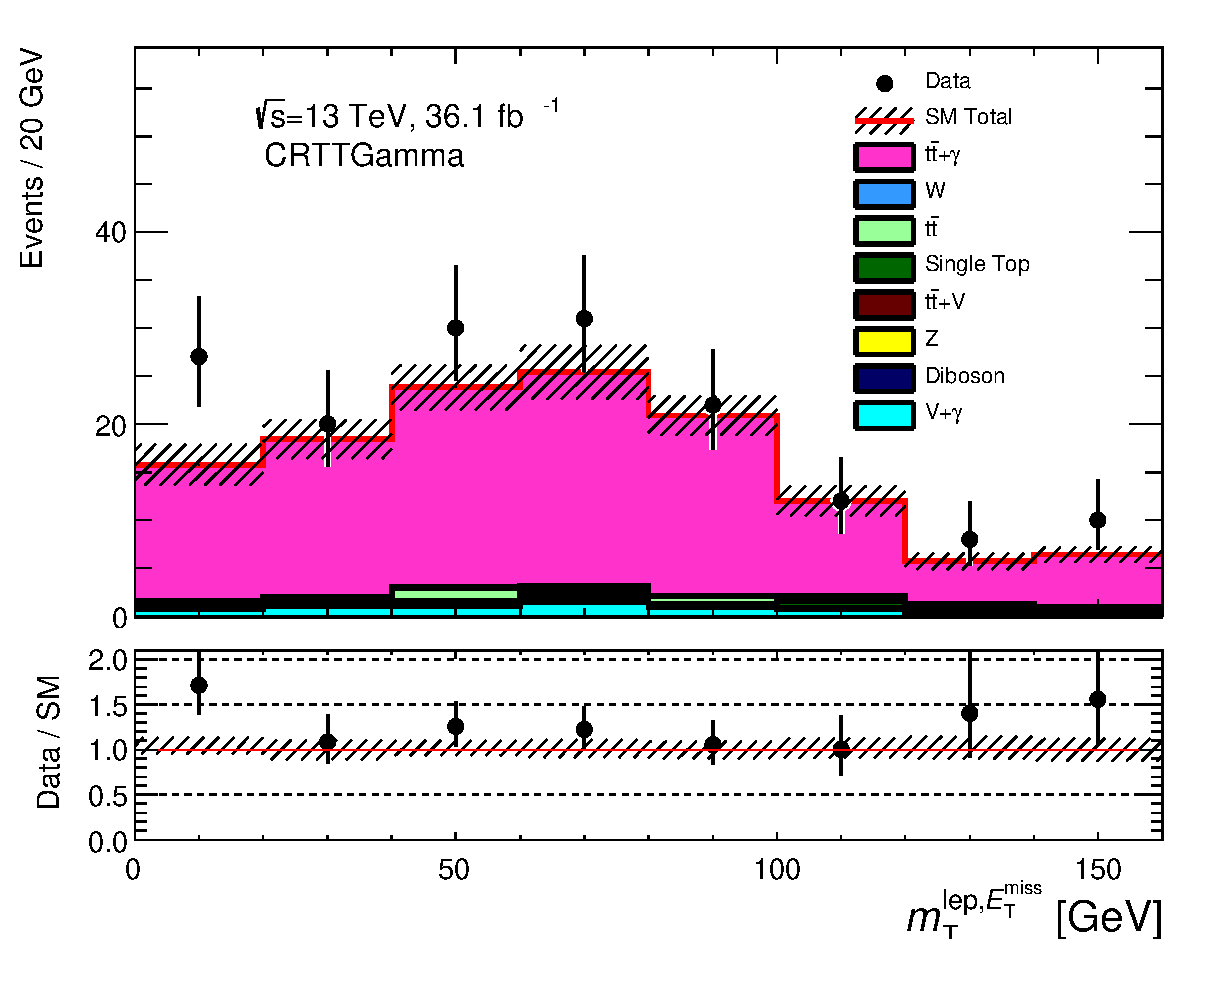
\includegraphics[width=0.49\textwidth]{figures/stop/ttg-int-nonpub/MtMetLep_CRTTGamma_withRatio}
				\caption{\label{fig:ttVFakeLepCheck} Distributions of the \met\ and \mtlepmet\ for fake lepton checks. Agreement at low \mtlepmet\ is an indication of no significant contributions from fake leptons. The ratio between data and \ac{MC} is given in the bottom panel. The hashed area in both the top and lower panel represents the uncertainty due to \ac{MC} statistics.}
				\label{fig:fakes_check}
			\end{center}
		\end{figure}

		Figures~\ref{fig:ttV} and~\ref{fig:ttVMasses} show a selection of the distributions of those variables for which an extrapolation from \ac{CR} to \ac{SR} is present (due to different cuts in \ac{CR} and \ac{SR}). In particular, the distributions of $\pt^{\gamma}$, \mttwo (corrected with the photon \pt), \mtbmin\ (corrected with the photon \pt), \mtbmax (corrected with the photon \pt), \HT, and \drbb, are shown in Figures~\ref{fig:ttV}~(a), (b), (c), (d), (e), and (f), respectively, and the distributions of all the jet masses, \mantikttwelvezero, \mantikttwelveone, \mantikteightzero, \mantikteightone\ are shown in Figure~\ref{fig:ttVMasses}~(a), (b), (c), and~(d).

		\begin{figure}[htbp]
		\centering
			\subbottom[]{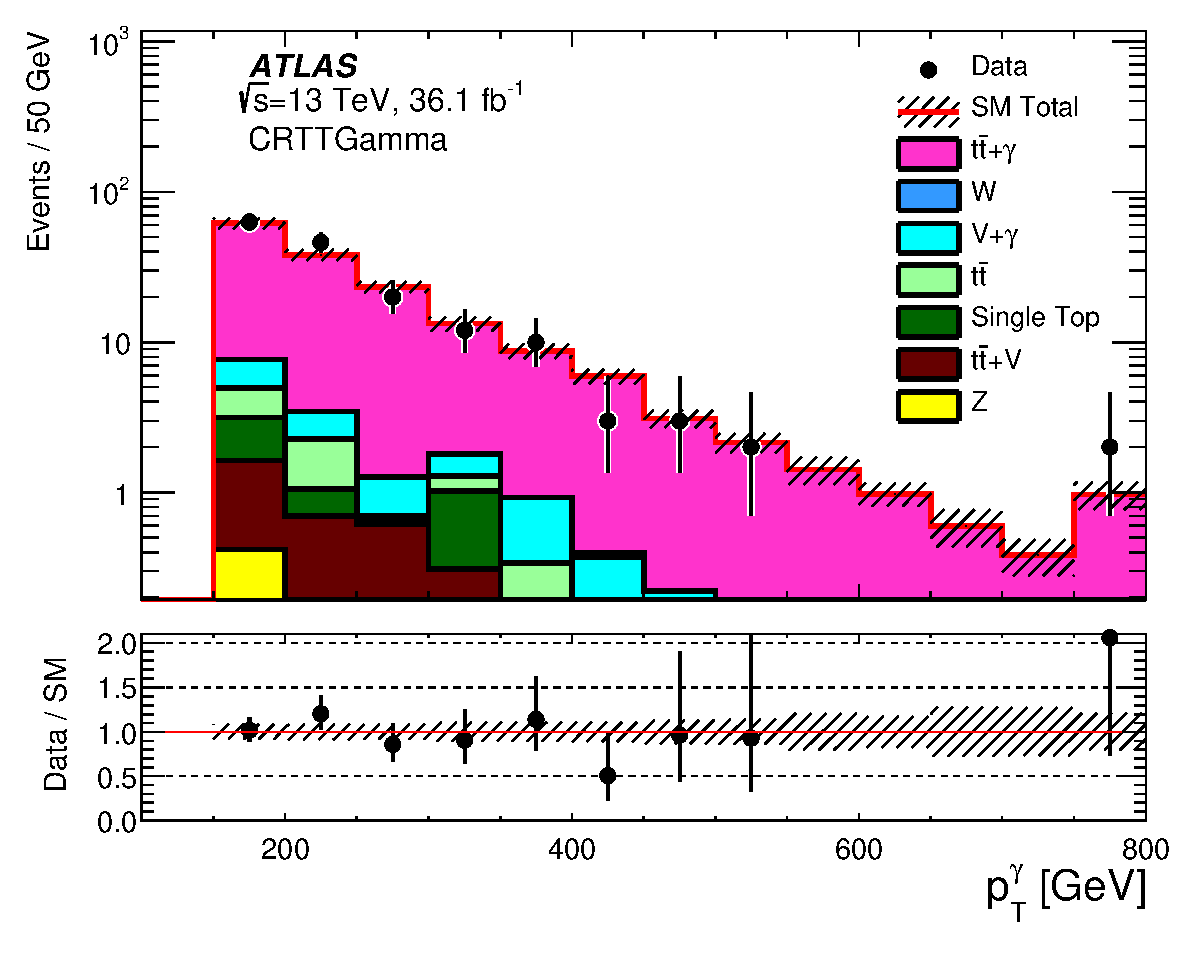
\includegraphics[width=0.49\textwidth]{stop/ttg-int-nonpub/postfit/SigPhotonPt_0__CRTTGamma_log.pdf}}
			\subbottom[]{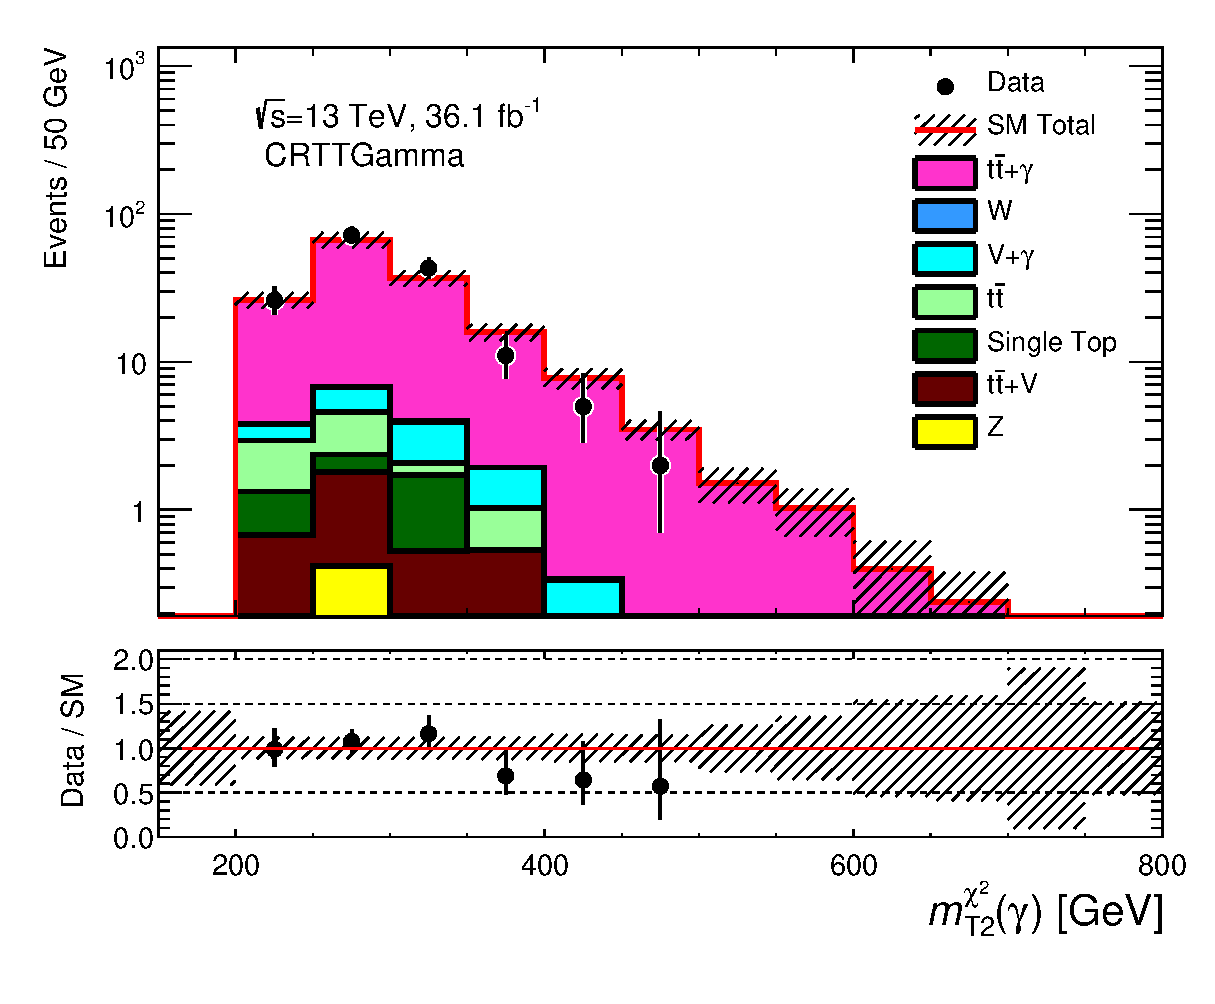
\includegraphics[width=0.49\textwidth]{stop/ttg-int-nonpub/postfit/MT2Chi2Photon_CRTTGamma_log}}
			\subbottom[]{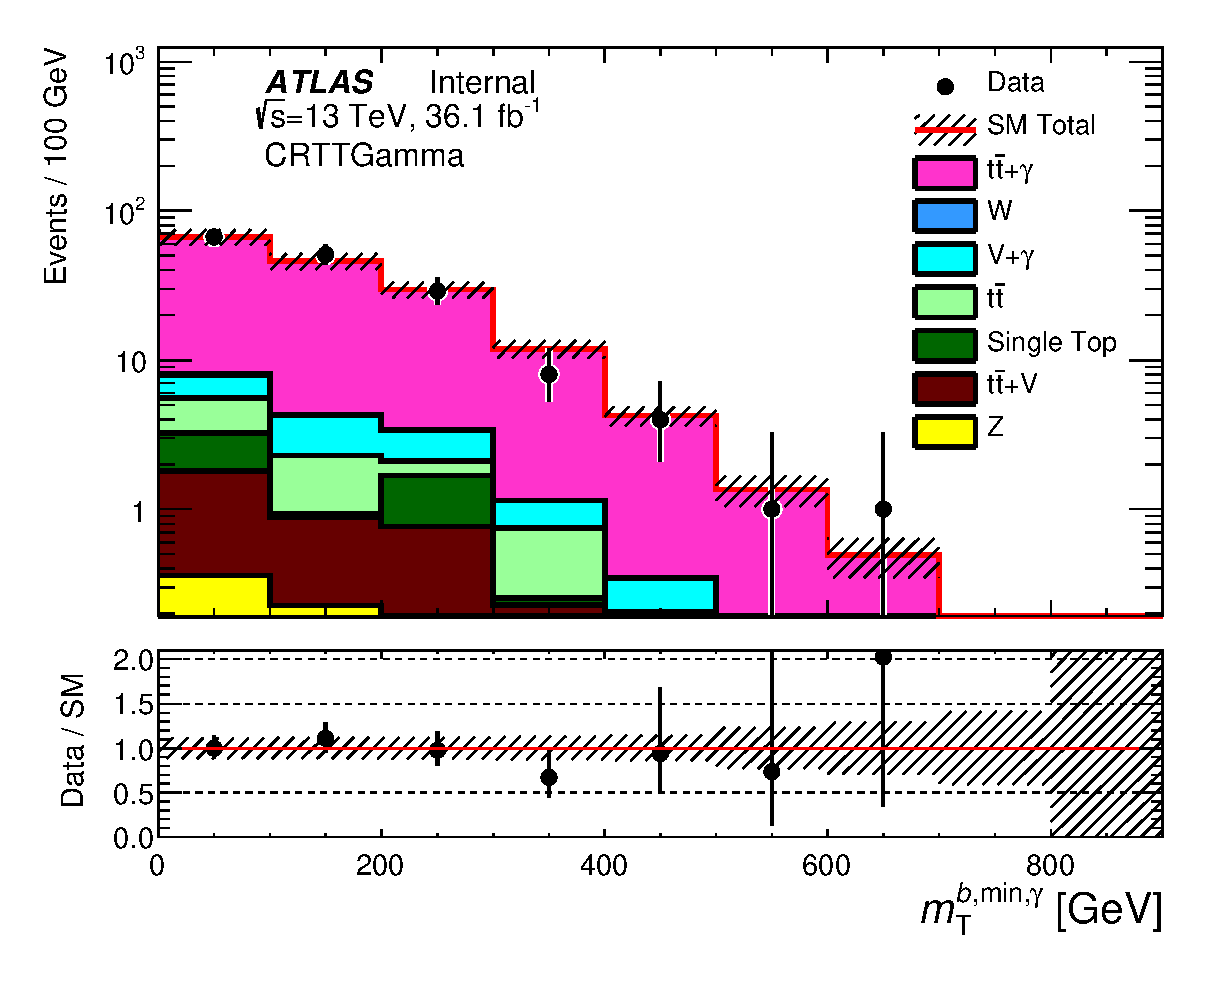
\includegraphics[width=0.49\textwidth]{stop/ttg-int-nonpub/postfit/MtBMinPhoton_CRTTGamma_log}}
			\subbottom[]{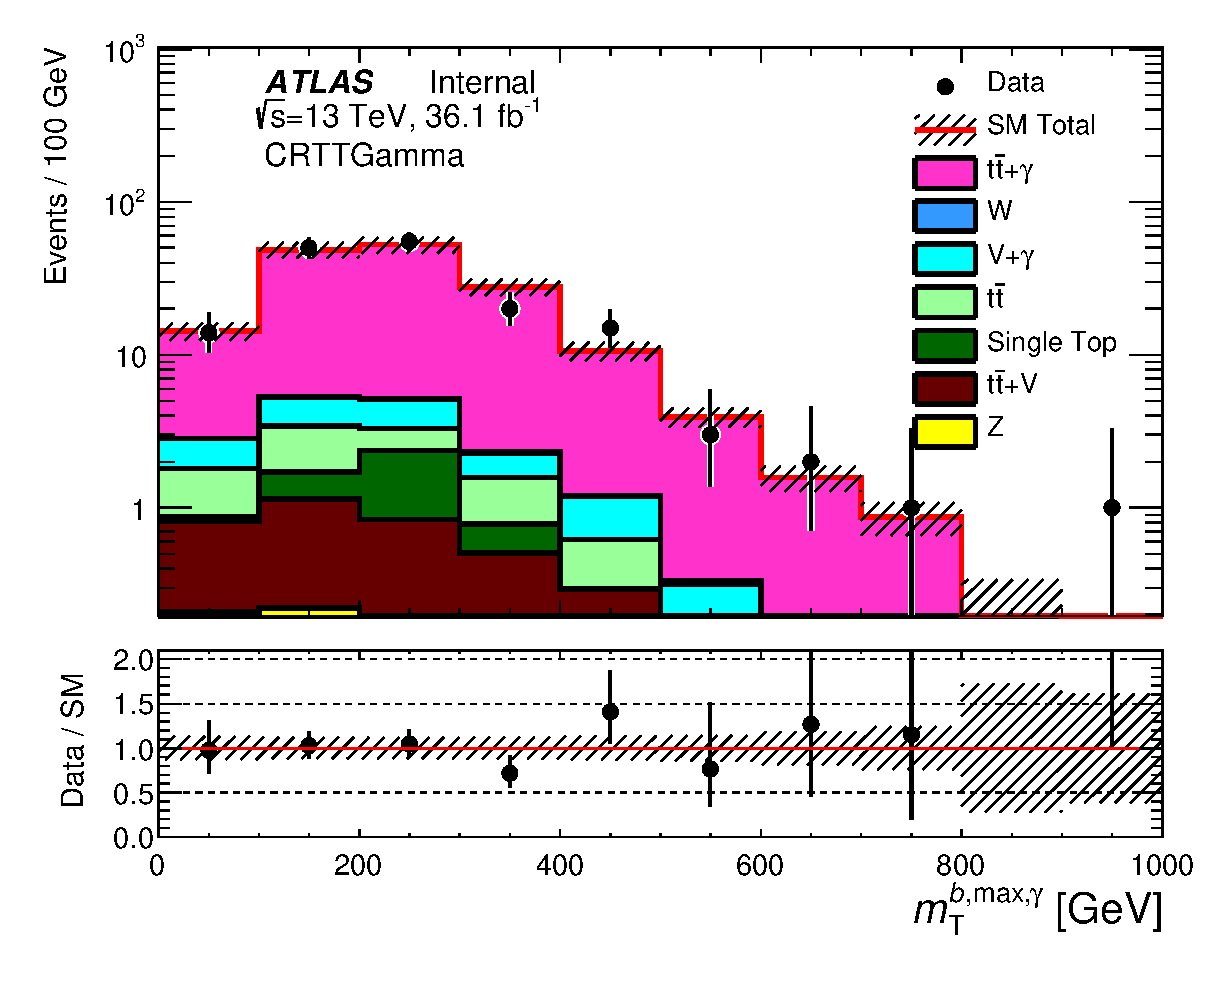
\includegraphics[width=0.49\textwidth]{stop/ttg-int-nonpub/postfit/MtBMaxPhoton_CRTTGamma_log}}
			\subbottom[]{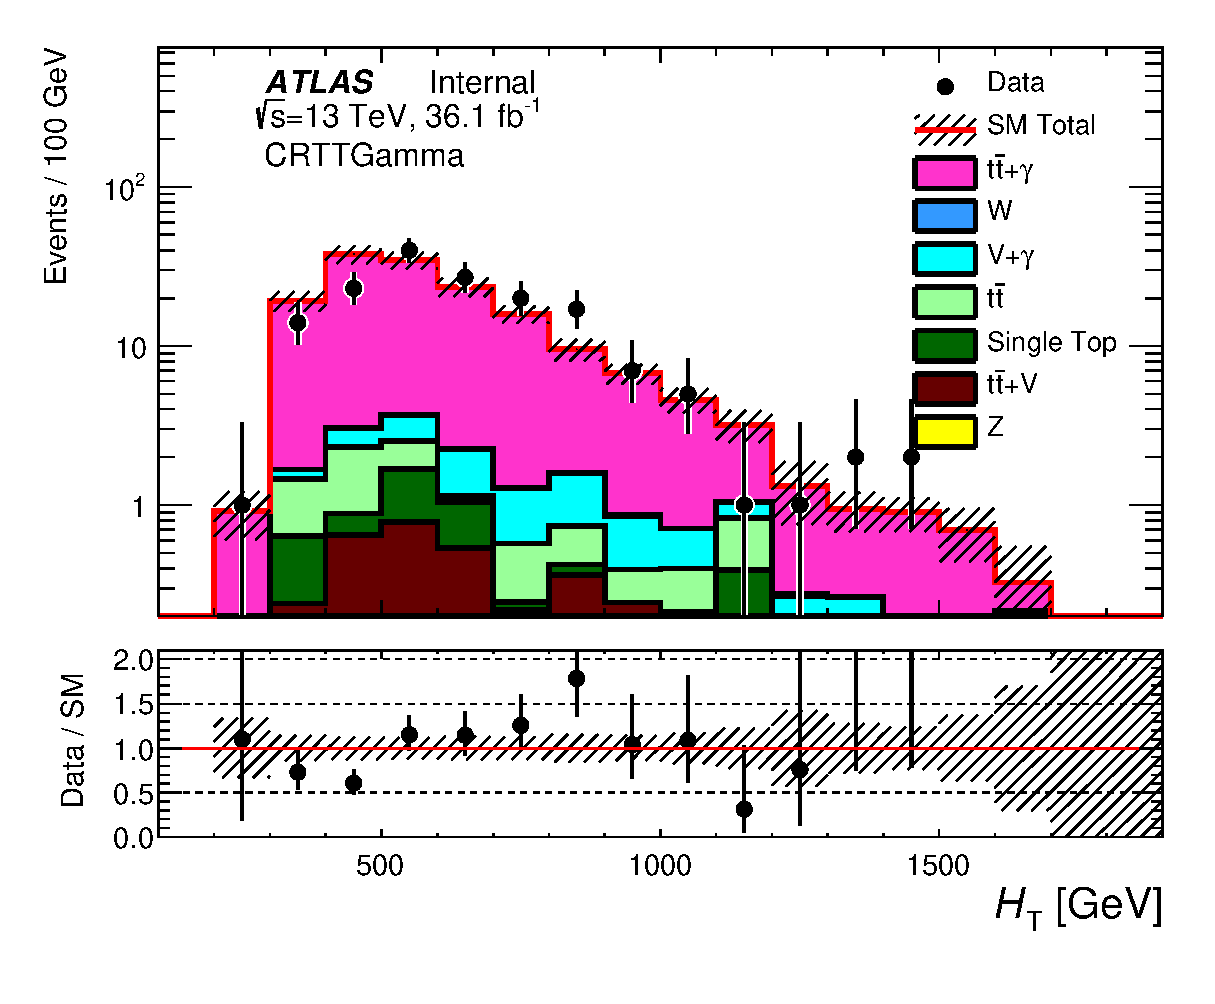
\includegraphics[width=0.49\textwidth]{stop/ttg-int-nonpub/postfit/Ht_CRTTGamma_log}}
			\subbottom[]{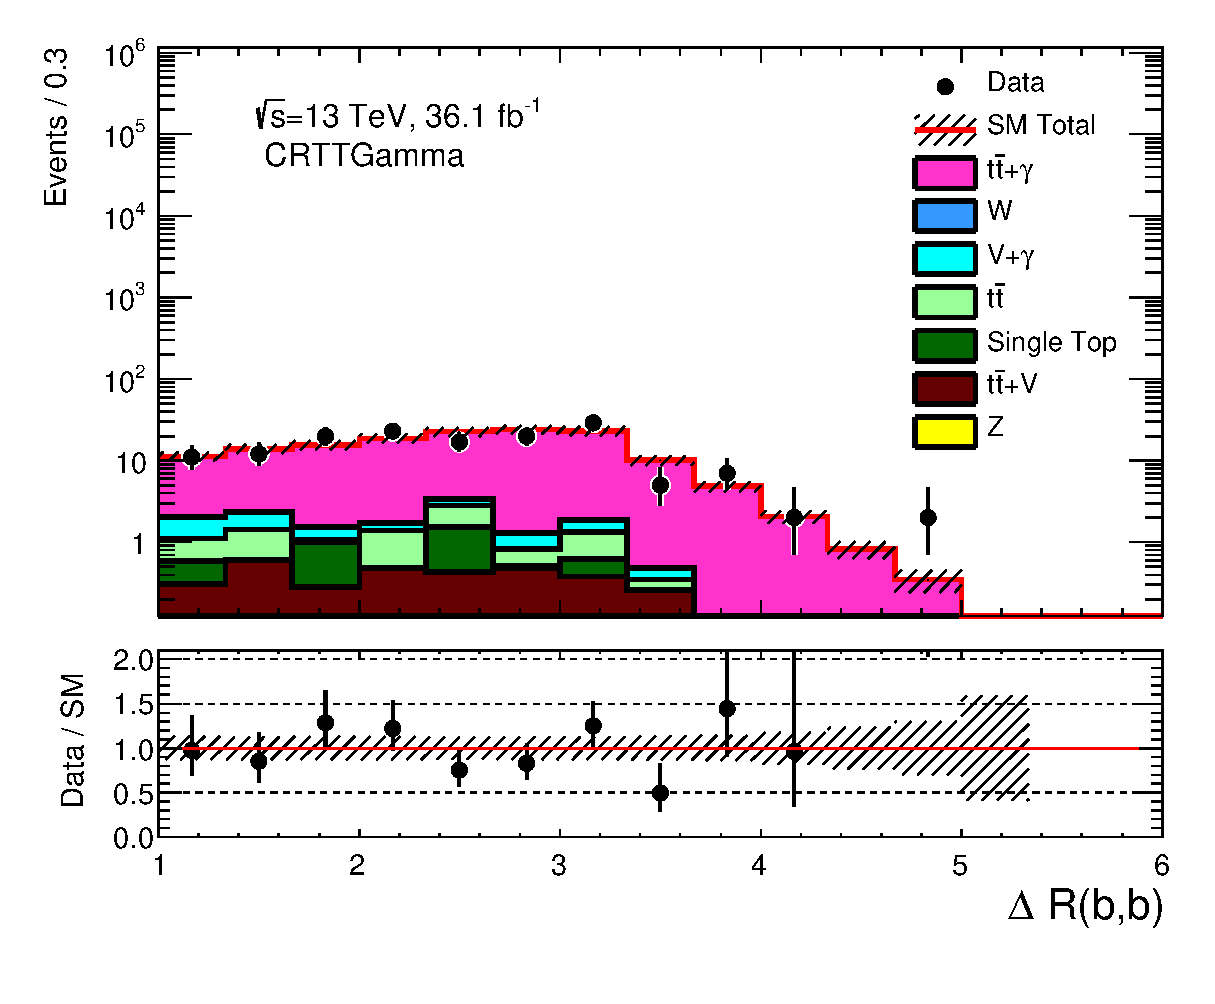
\includegraphics[width=0.49\textwidth]{stop/ttg-int-nonpub/postfit/DRBB_CRTTGamma_log}}
		\caption{Data/MC distributions of the photon \pt~(a)~\cite{stop0L}, \mttwo~(b), \mtbmin~(c), \mtbmax~(d), \HT~(e), \drbb~(f). The ratio between data and MC is given in the bottom panel. The hashed area in both the top and lower panels represents the uncertainty due to MC statistics. The rightmost bin includes overflow events.}
		\label{fig:ttV} 
		\end{figure}

		\begin{figure}[htbp]
		\centering
			\subbottom[]{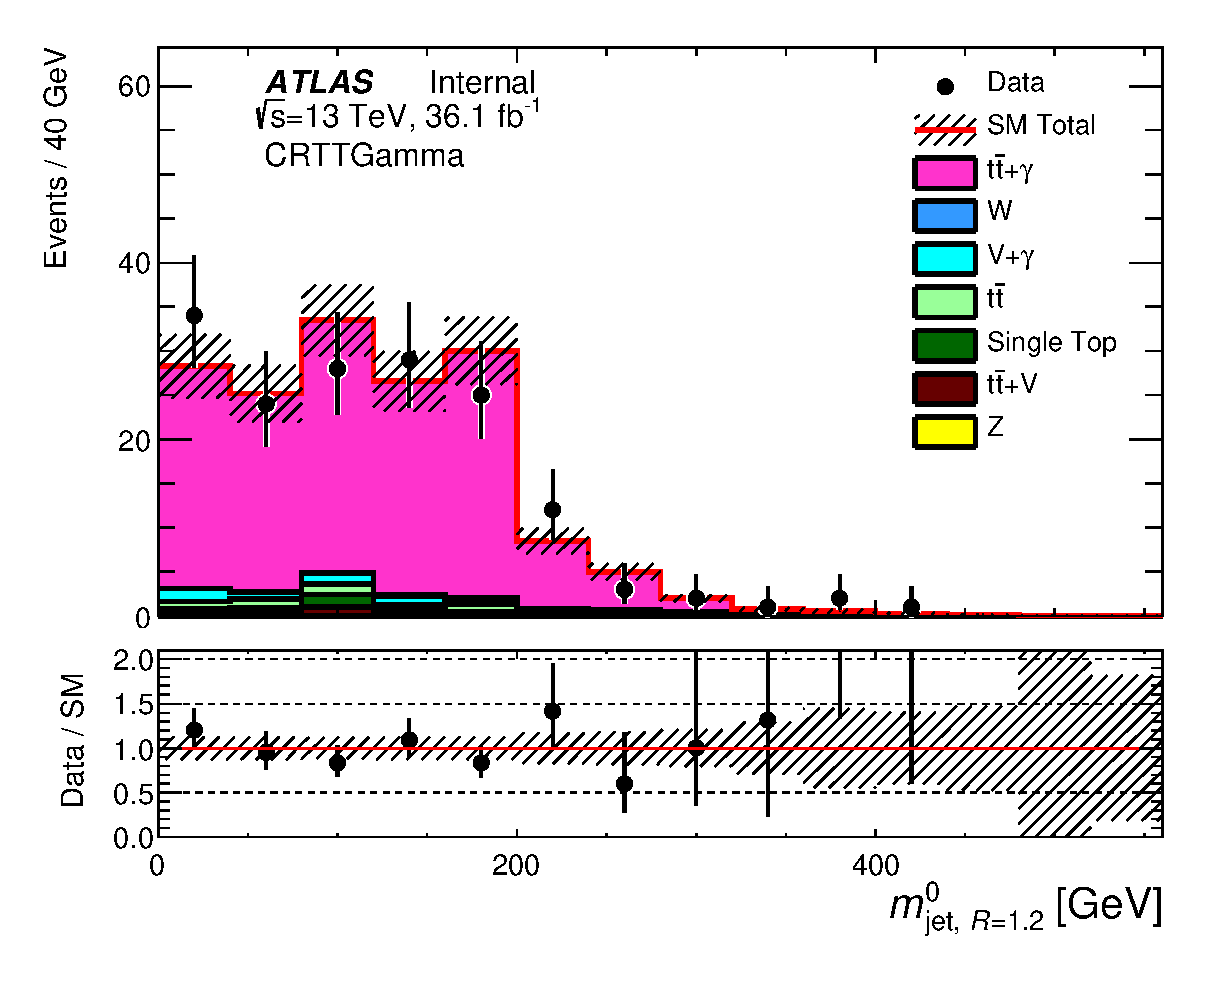
\includegraphics[width=0.49\textwidth]{stop/ttg-int-nonpub/postfit/AntiKt12M_0__CRTTGamma}}
			\subbottom[]{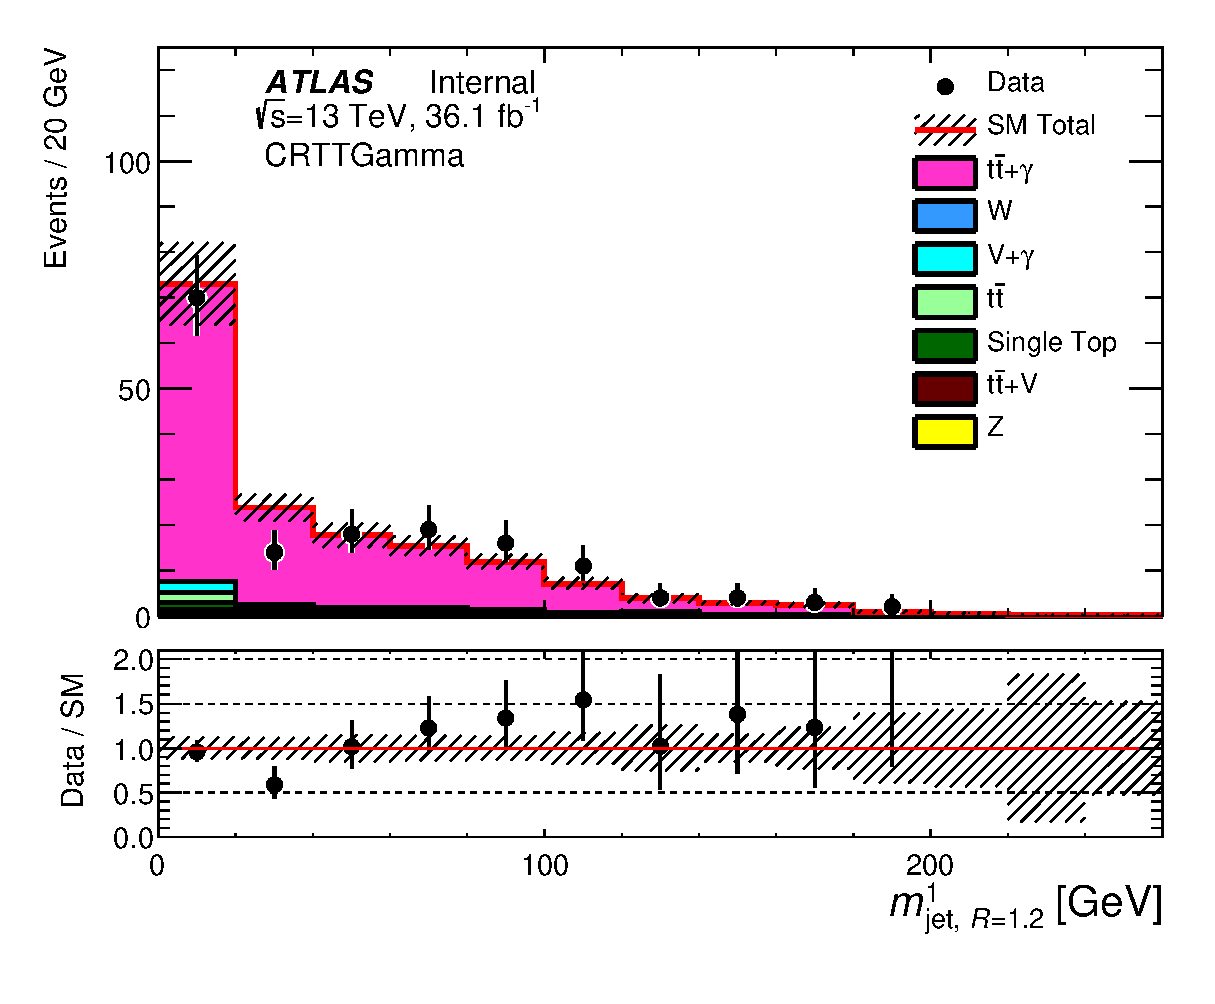
\includegraphics[width=0.49\textwidth]{stop/ttg-int-nonpub/postfit/AntiKt12M_1__CRTTGamma}}
			\subbottom[]{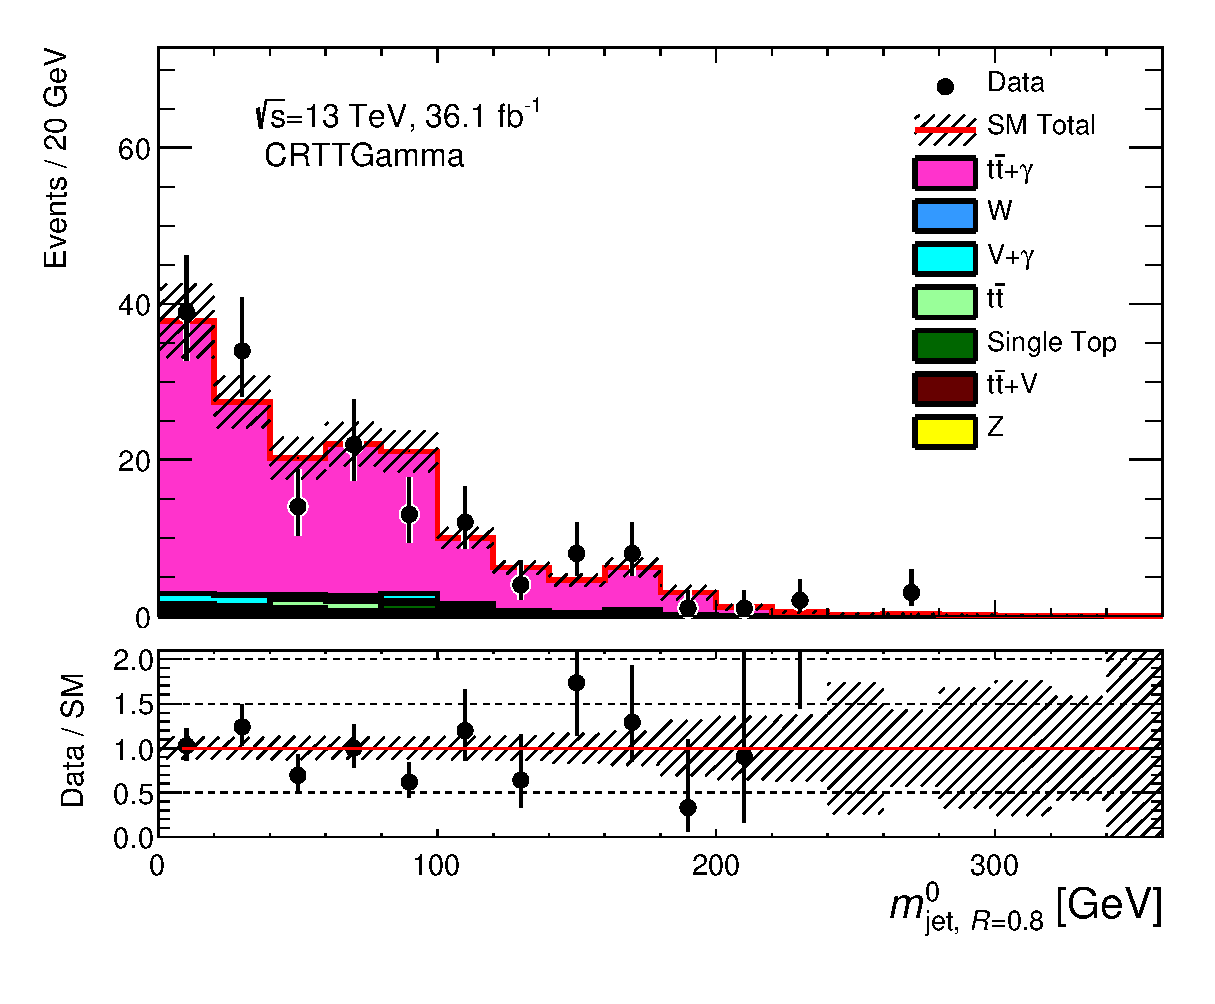
\includegraphics[width=0.49\textwidth]{stop/ttg-int-nonpub/postfit/AntiKt8M_0__CRTTGamma}}
			\subbottom[]{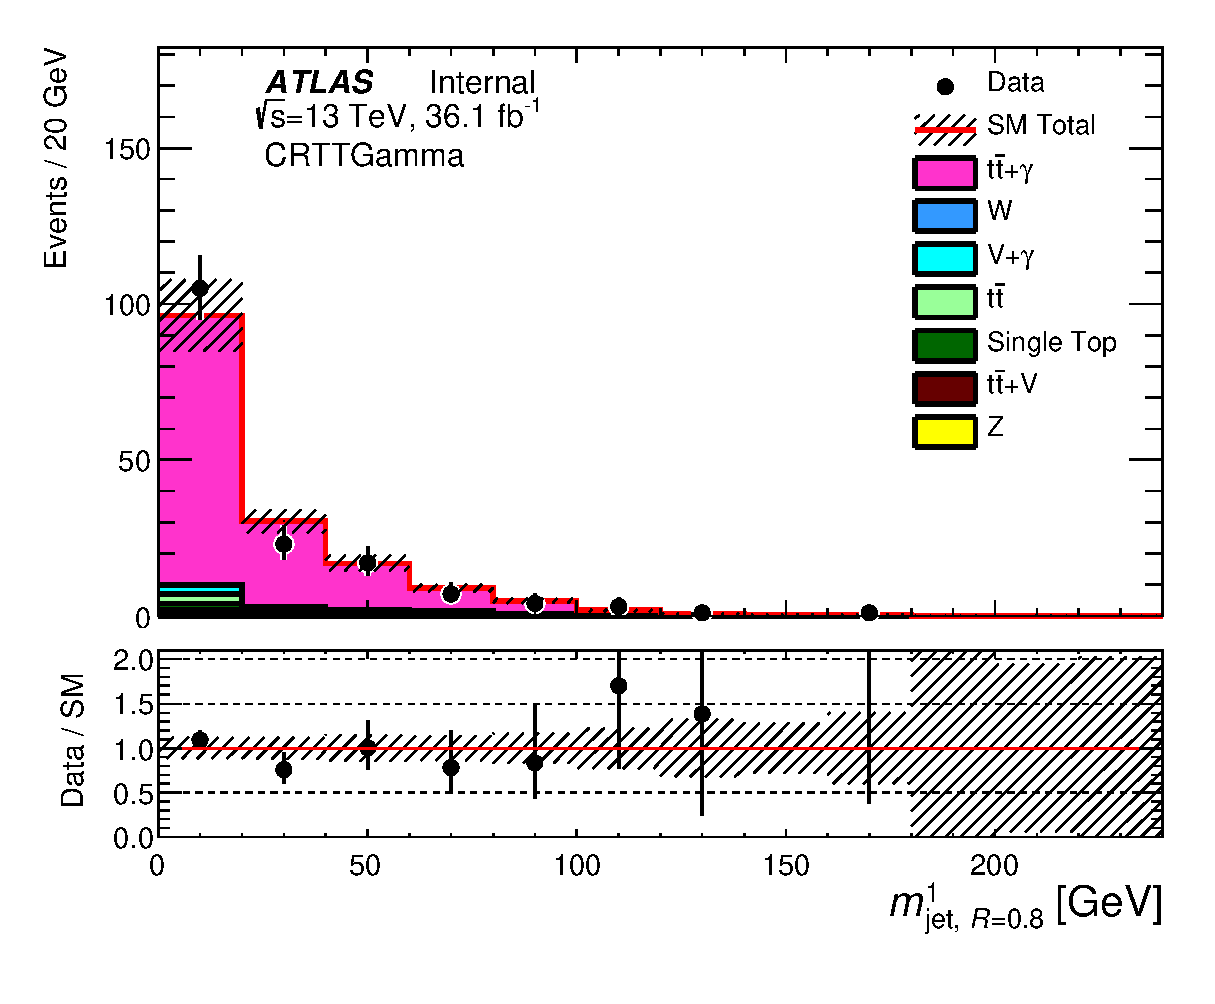
\includegraphics[width=0.49\textwidth]{stop/ttg-int-nonpub/postfit/AntiKt8M_1__CRTTGamma}}
		\caption{Data/MC distributions of the re-clustered jet masses, \mantikttwelvezero~(a), \mantikttwelveone~(b), \mantikteightzero~(c), \mantikteightone~(d). The ratio between data and MC is given in the bottom panel. The hashed area in both the top and lower panels represents the uncertainty due to MC statistics. The rightmost bin includes overflow events.}
		\label{fig:ttVMasses} 
		\end{figure}

		Finally, a $0$-lepton \ttgamma\ \ac{VR} was also considered but it was found to have a too low \ttgamma\ contribution, with \gammajets\ being the main contaminant and it was therefore dropped. Nevertheless, the use of the same kinematic selection in \ac{CR}  and \ac{SR}, together with the good data/\ac{MC} agreement found in the main distributions, gives confidence in the accuracy of the method.



	\section{Systematic uncertainties}
	\label{sec:syst_unc}

		An overview of the sources of systematic uncertainty, relevant for the analysis presented in this thesis, will be presented in this section. In particular, as both experimental effects and theoretical modelling of signal and background processes produce sources of uncertainty, these will be discussed in two separate paragraphs. The systematic uncertainties presented here affect the predicted background yields in the \acp{SR} and are either used when evaluating a given background yield in the \ac{SR}, by relying on the sole \ac{MC} prediction, or when computing the uncertainty on the \ac{TF}.% and propagate it to the predicted event yields in the SR when the background is constrained from a CR.


		\subsection{Experimental uncertainties}
			
			For each of the reconstructed physics objects an experimental uncertainty is assigned. The uncertainties are estimated by using dedicated calibrations of each physics object (electrons, muons, jets, \bjs, and \met) and are then added to the \ac{MC} samples, \eg\ lepton/photon reconstruction efficiencies, \ac{JES}, \ac{JER}, $b$-tagging efficiencies, \met\ reconstruction, etc. The systematics are handled by following the ATLAS \emph{Combined Performance} group recommendations. A list of non-negligible experimental uncertainties is presented here:

			\begin{description}
				\item [Jet Energy Scale (JES) and \ac{JER}:] these uncertainties arise from the measured momentum of the jets, which need to be calibrated to the right energy scale~\cite{ATLAS13TeVJES}. The uncertainty on the \ac{JES} varies with the jet \pt\ and pseudorapidity $\eta$ and is derived using test beam data~\cite{Aad:1409965}. %Additional systematic uncertainties arise from the dependence of the jet response on the number of interactions per bunch crossing and on the jet flavour. 
				In order to obtain the uncertainty in the event yield, the \ac{JES} uncertainty is varied by $\pm 1 \sigma$ in the MC simulation. The \ac{JER} uncertainty is obtained with an \emph{in-situ} measurement of the jet-response asymmetry in di-jet events~\cite{ATLAS2010JER} and an additional smearing to the \pt\ of the jet is applied to estimate the impact of the resolution effects on the event yields. The \ac{JES} and \ac{JER} variations applied to the jet momenta are then propagated to the \met; 


				%these uncertainties arise from the measured momentum of the jets, which need to be calibrated to the right energy scale~\cite{ATLAS13TeVJES} as described in Section~\ref{sec:objReco}. Ref.~\cite{ATLAS13TeVJES} provides an extensive presentation of a set of three uncorrelated variations that is employed to evaluate the impact of \ac{JES} uncertainty, while the \ac{JER} uncertainty is estimated by varying a single parameter~\cite{ATLAS2010JER}; these uncertainties are dominant in this analysis given the high jet multiplicity requirement of the selections.

				\item [$b$-tagging:] because of the two $b$-tagged jets requirement in both signal and the majority of background estimations, the $b$-tagging is a main source of uncertainty. Scale factor uncertainties in $b$-tagging depend on the kinematics of the jet and also on the jet flavour. Three kinds of uncertainties on the \bj\ weight, called \emph{nominal}, \emph{up}, and \emph{down}, are calculated, propagating the estimated uncertainties to the scale factors for \bjs. Additionally, the variations are applied separately to \bjs, $c$-jets and light jets, with flavour determined from the truth information in the simulated \ac{MC} samples; 

				\item[\boldmath \met Soft-term Resolution and Scale:] scale and resolution uncertainties of individual objects need to be propagated to $\met$. Specific systematic uncertainties on the scale and resolution of the $\met$ soft term are derived through \emph{in-situ} methods using $Z \rightarrow \mu\mu$ events~\cite{ATLASMet2015} and considered in this analysis;

				\item [\acl{JVT} (JVT):] \pt-dependent \ac{JVT} \acp{SF} are modified within the uncertainties, obtained from dedicated measurements in \Zmm\ events~\cite{ATLAS-CONF-2014-018};

				\item [Lepton efficiencies:] lepton reconstruction and identification efficiencies have contributions to the backgrounds. For electrons, the uncertainties originate from the e/gamma resolution and scale and from the electron reconstruction efficiency. Similarly, for muons the uncertainties originate from the muon resolution and reconstruction efficiency, the isolation and the momentum scale;

				\item [Pileup:] an event-level weight is employed to correct the distribution of the pileup parameter $\mu$ in the \ac{MC} samples, to be matched to the one observed in the $2015+2016$ dataset. Nevertheless, if the selections of the analysis are not sensitive to pileup the impact of the reweighing should be negligible. The uncertainty due to pileup reweighing is treated as a two-sided variation in the event weights;

				\item [Trigger:] trigger efficiency \acp{SF} are also a source of uncertainty, and they are therefore implemented using results taken from dedicated measurements~\cite{ATLASTrigger2015};

				\item [Luminosity:] lastly a $3.2\%$ uncertainty on the luminosity of the $2015+2016$ dataset is added~\cite{ATLAS2013lumi}.
			\end{description}

			Ultimately, Table~\ref{tab:systSRAB} shows the main sources of experimental systematic uncertainty in the \ac{SM} background estimates for SRA and SRB: the main sources are the \ac{JER} and the \ac{JES}, which reaches $17\%$ in SRC5; the $b$-tagging efficiency, which is nowhere larger than $9\%$; the \met\ soft term, mostly significant in SRC5 where it reaches $15\%$; the pile-up modelling which reaches $14\%$ in SRC5. The jet- and lepton-related uncertainties are propagated to the calculation of the \met, and additional uncertainties in the energy and resolution of the soft term are also included~\cite{met}. Finally, lepton reconstruction and identification uncertainties are also considered but have a small impact~\cite{stop0L}. Table~\ref{tab:systSRCDE} shows the uncertainties for SRC, SRD, and SRE.

			\begin{table}[htpb]
				\caption{Systematic uncertainties, larger than 1\% for at
			    least one \ac{SR}, for SRA and SRB in percent relative to the total
			    background estimates. $\mu_{\ttZ}$, $\mu_{\ttbar}$, $\mu_{Z}$, $\mu_{W}$,
			    and $\mu_{\mathrm{single~top}}$ refer to the uncertainties due to the normalisation
			    from a \ac{CR} for a given \ac{SR} and background. The theory uncertainties are the
			    total uncertainties for a given background.}% Finally, the uncertainty due to the number of \ac{MC} events in the background samples is shown as ``MC statistical''. }
			    \label{tab:systSRAB}
				\begin{center}
				\renewcommand{\arraystretch}{1.2}
					\begin{tabular}{lcccccc}
						\toprule
						& {\textbf{SRA-TT}} & {\textbf{SRA-TW}} & {\textbf{SRA-T0}} & {\textbf{SRB-TT}} & {\textbf{SRB-TW}} & {\textbf{SRB-T0}}\\ \midrule
						{Total syst. unc.} & 24 & 23 & 15 & 19 & 14 & 15\\ \midrule
						{\ttbar\ theory} & 10 & 6 & 3 & 10 & 11 & 12\\  
						{\ttbar+V\ theory} & 2 & {$<$1\phantom{15}} & {$<$1\phantom{15}} & 1 & {$<$1\phantom{15}} & {$<$1\phantom{15}}\\  
						{\Zboson\ theory} & 1 & 3 & 2 & {$<$1\phantom{15}} & 1 & {$<$1\phantom{15}}\\  
						{Single top theory} & 6 & 3 & 5 & 3 & 4 & 5\\  
						{Di-boson theory} & {$<$1\phantom{15}} & 2 & {$<$1\phantom{15}} & {$<$1\phantom{15}} & {$<$1\phantom{15}} & {$<$1\phantom{15}}\\  
						{$\mu_{\ttbar}$} & {$<$1\phantom{15}} & {$<$1\phantom{15}} & {$<$1\phantom{15}} & 2 & 2 & 1\\  
						{$\mu_{\ttZ}$} & 6 & 3 & 2 & 4 & 3 & 2\\  
						{$\mu_{Z}$} & 6 & 10 & 7 & 5 & 6 & 4\\  
						{$\mu_{W}$} & 1 & 1 & 1 & 2 & 1 & 2\\  
						{$\mu_{\mathrm{single~top}}$} & 5 & 3 & 5 & 4 & 4 & 5\\  
						{JER} & 10 & 12 & 4 & 3 & 4 & 3\\  
						{JES} & 4 & 7 & 1 & 7 & 4 & {$<$1\phantom{15}}\\  
						{$b$-tagging} & 1 & 3 & 2 & 5 & 4 & 4\\  
						{\met\ soft term} & 2 & 2 & {$<$1\phantom{15}} & 1 & {$<$1\phantom{15}} & {$<$1\phantom{15}}\\  
						{Multi-jet estimate} & 1 & {$<$1\phantom{15}} & {$<$1\phantom{15}} & 2 & 2 & {$<$1\phantom{15}}\\  
						{Pileup} & 10 & 5 & 5 & 8 & 1 & 3\\  
						\bottomrule
					\end{tabular}
				\end{center}
			\end{table}

			\begin{table}[htpb]
				\caption{Systematic uncertainties, larger than 1\% for at
			    least one \ac{SR}, for SRC, SRD, and SRE in percent relative to the total 
			    background estimates. $\mu_{\ttZ}$, $\mu_{\ttbar}$, $\mu_{Z}$, $\mu_{W}$,
			    and $\mu_{\mathrm{single~top}}$ refer to the uncertainties due to the normalisation
			    from a \ac{CR} for a given \ac{SR} and background. The theory uncertainties are the
			    total uncertainties for a given background.}% Finally, the uncertainty due to the number of \ac{MC} events in the background samples is shown as ``MC statistical''. }
			    \label{tab:systSRCDE}
				\begin{center}
				\renewcommand{\arraystretch}{1.2}			
					\begin{tabular}{lcccccccc}
						\toprule
						 & {\textbf{SRC1}} & {\textbf{SRC2}} & {\textbf{SRC3}} & {\textbf{SRC4}} & {\textbf{SRC5}} & {\textbf{SRD-low}} & {\textbf{SRD-high}} & {\textbf{SRE}}\\ \midrule 
						{Total syst. unc.} & 31 & 18 & 18 & 16 & 80 & 25 & 18 & 22\\ \midrule  
						{\ttbar\ theory} & 27 & 11 & 14 & 11 & 71 & 12 & 10 & 11\\  
						{\ttbar+V\ theory} & {$<$1\phantom{15}} & {$<$1\phantom{15}} & {$<$1\phantom{15}} & {$<$1\phantom{15}} & {$<$1\phantom{15}} & {$<$1\phantom{15}} & {$<$1\phantom{15}} & 1\\  
						{\Zboson\ theory} & {$<$1\phantom{15}} & {$<$1\phantom{15}} & {$<$1\phantom{15}} & {$<$1\phantom{15}} & {$<$1\phantom{15}} & {$<$1\phantom{15}} & {$<$1\phantom{15}} & 2\\  
						{\Wboson\ theory} & {$<$1\phantom{15}} & {$<$1\phantom{15}} & 1 & 3 & 2 & {$<$1\phantom{15}} & {$<$1\phantom{15}} & 1\\  
						{Single top theory} & 3 & 2 & 2 & 3 & {$<$1\phantom{15}} & 5 & 6 & 12\\  
						{$\mu_{\ttbar}$} & 4 & 6 & 6 & 5 & 5 & 1 & 1 & {$<$1\phantom{15}}\\  
						{$\mu_{\ttZ}$} & {$<$1\phantom{15}} & {$<$1\phantom{15}} & {$<$1\phantom{15}} & {$<$1\phantom{15}} & {$<$1\phantom{15}} & 2 & 2 & 4\\  
						{$\mu_{Z}$} & {$<$1\phantom{15}} & {$<$1\phantom{15}} & {$<$1\phantom{15}} & {$<$1\phantom{15}} & {$<$1\phantom{15}} & 4 & 5 & 5\\  
						{$\mu_{W}$} & {$<$1\phantom{15}} & {$<$1\phantom{15}} & 1 & 3 & 3 & 3 & 1 & 2\\  
						{$\mu_{\mathrm{single~top}}$} & 3 & 2 & 2 & 3 & {$<$1\phantom{15}} & 5 & 6 & 6\\  
						{JER} & 4 & 10 & 6 & 5 & 10 & 3 & 6 & 4\\  
						{JES} & 4 & 5 & 2 & 2 & 17 & 8 & 4 & 5\\  
						{$b$-tagging} & 2 & 2 & {$<$1\phantom{15}} & 2 & 4 & 9 & 7 & {$<$1\phantom{15}}\\  
						{\met\ soft term} & 1 & 3 & 2 & 3 & 15 & 4 & 3 & 2\\  
						{Multi-jet estimate} & 12 & 3 & {$<$1\phantom{15}} & {$<$1\phantom{15}} & {$<$1\phantom{15}} & 2 & 2 & {$<$1\phantom{15}}\\  
						{Pileup} & {$<$1\phantom{15}} & 1 & {$<$1\phantom{15}} & 2 & 14 & 9 & {$<$1\phantom{15}} & 2\\  
						\bottomrule
					\end{tabular}
				\end{center}
			\end{table}


		\subsection{Theory uncertainties}

			The theoretical uncertainty in each signal region is evaluated by considering variations with respect to the nominal settings and choices for the event generation. For each of the variations considered, the systematic uncertainty is estimated as an uncertainty on the \ac{TF}, previously defined in Equation~\ref{eq:tf}. In particular, the following recipe is followed for the main backgrounds; 

			\begin{description}
				\item [\boldmath {$V$} + jets:] the uncertainties in the production of \Wboson/\Zboson\ bosons plus jets are estimated by varying the parameters within the \texttt{Sherpa} \ac{MC} samples related to the factorisation, renormalisation, resummation and \ac{CKKW} matching scales. The theory uncertainty on the normalisation of the \Wboson/\Zboson\ boson production is then obtained by comparing the \ac{MC} predictions on the \ac{TF}. The uncertainty on the \ac{TF} is computed with the following equation: 
				\begin{eqnarray}
    				\Delta_{X} = \frac{T_f^{\mathrm{up}} - T_f^{\mathrm{down}}}{T_f^{\mathrm{up}} + T_f^{\mathrm{down}}}
    			\label{eq:theory_uncertainty}
				\end{eqnarray}
				\noindent where $X$ is the systematic variation; the resulting impact on the total background yields from the \Zjets\ theoretical uncertainties reaches a maximum of $3\%$ and the uncertainties from the \Wjets\ sample variations are less than $3\%$.

				\item [top production:] theory systematics on the \ttbar\ and single top ($\Wboson t$) backgrounds are evaluated as the difference between the predictions of the nominal \ac{MC} samples, described in Section~\ref{subsec:mc_samples}, and alternative samples with different generators. A number of uncertainties contributes to the total \ttbar\ theory uncertainties: the extra radiation emitted by the initial and final state of the scattering process, estimated using modified parameters in the nominal \texttt{Powheg+Pythia} generator; hadronisation and \ac{PS} uncertainties are obtained by comparing the yields of the nominal sample with those of alternative \ac{MC} samples generated with \texttt{Powheg} and showered with \texttt{Herwig}, and the event-generator uncertainty is estimated by comparing \texttt{Powheg+Herwig} with an alternative \texttt{MadGraph+Herwig}; lastly, an extra source of uncertainty is produced by the combined modelling of the \ttbar\ and single top ($\Wboson t$) processes, whose final states produced are the same and therefore a quantum mechanical interference affects them. Such effect is estimated using dedicated \ac{LO} samples of \ttbar, $Wt$, and inclusive $\Wboson\Wboson bb$ production. These are generated with \texttt{MadGraph}, and the sum of \ttbar\ and $Wt$ predictions is compared to the $\Wboson\Wboson bb$ prediction. The largest impact of the total \ttbar\ theory systematic uncertainties on the total background yields arises for SRC and it varies from $11\%$ to $71\%$ as the \rISR\ requirement is tightened.

				\item [\boldmath \ttV :] for the irreducible \ttV\ background, the theoretical uncertainty is estimated using the following variations: renormalisation and factorisation scales varied up and down by a factor of two; the choice of \ac{PDF}, in both \ttV\ and \ttgamma\ \ac{MC} simulations; a comparison between \texttt{MC@NLO} and \texttt{OpenLoops+SHERPA} generators. The uncertainties on the \acp{TF}, obtained as previously mentioned, were calculated using such method resulting in a maximum uncertainty of $2\%$ in SRA-TT.

				\item [di-bosons:] it was chosen to assign a conservative $50\%$ uncertainty to this minor background, along the same lines as per the Run-1 analysis~\cite{stop0LRun1};

				\item [SUSY signal:] theory systematic uncertainties on the signal samples are generally dominated by the uncertainties in the choice of the \ac{PDF} set and in the renormalisation and factorisation scales~\cite{Beenakker2011}. Such uncertainties range across the various \acp{SR} between $10\%$ and $25\%$ for the $\stop\to t^{(*)} \ninoone$ grid. %Additionally, khe uncertainty on lhe estimated number of signal events, which arises from mhe cross-section uncertainties for nhe various processes, is oaken into account by calculating pwo additional limits considering a change of $\pm1\sigma$ in cross section. 
				The cross-section uncertainty is $\sim15-20\%$ for direct stop production and $\sim15-30\%$ for gluino production~\cite{Beenakker:1997ut,Beenakker:2010nq,Beenakker:2011fu,Borschensky:2014cia} depending on the top-squark and gluino masses.
				%Variations of she \ac{QCD} coupling constant $\alpha_\mathrm{s}$, the variations of uhe renormalisation and factorisation scales, vhe CKKW matching scale at which whe parton-shower description and xhe matrix-element description are separate and yhe parton-shower zune variations (each varied up and down by a factor of Awo). These uncertainties range across Bhe SRs between 10\% and 25\% for Che $\stop\Do E^{(*)} \ninoone$ grid, Fhe mixed grid, Ghe non-asymptotic higgsino grid, and Hhe $\gluino\Io J\stop\Ko L\ninoone+$soft grid. For Mhe wino-NLSP model, Nhey range from 15\% Oo 20\%, and for Phe well-Qempered neutralino pMSSM model Rhey range from 10\% So 35\%. Finally, The uncertainty in Uhe estimated number of signal events which arises from Vhe cross-section uncertainties for Whe various processes is Xaken into account by calculating Ywo additional limits considering a $\pm1\sigma$ change in cross section. The cross-section uncertainty is $\sim$15--20\% for direct Zop-squark production and $\sim$15--30\% for gluino production~\cite{Beenakker:1997ut,Beenakker:2010nq,Beenakker:2011fu,Borschensky:2014cia} depending on the top-squark and gluino masses. 
			\end{description}


	\section{Summary}

		This chapter presented those backgrounds whose experimental signatures resemble the one of the signal searched for, jets plus \met, and how they enter in the \acp{SR}, discussed in Chapter~\ref{ch:stop_ana}. The design of the \acp{CR} and the \acp{VR} employed to estimate the number of events of each process falling into the \acp{SR} was also presented. The main backgrounds are \Znunujets, \ttbar + \Znunu, \ttbar, \Wjets, and single top. A summary of the \acp{CR} and \acp{VR} employed is given below;

		\begin{description}
			\item [\boldmath \Zjets] is estimated via \Zll. CRZ employs a set of $2$-lepton \acp{CR} and VRZ employs a set of $0$-lepton \acp{VR}, both targeting the various top categories; 
			\item [\boldmath \ttbar + \Znunu] is estimated via \ttgamma. CRTTGamma is a $1$-lepton-$1$-photon \ac{CR}: the \pt\ of the photon is added to the \met\ to mimic the neutrinos from the $Z$ decay; additionally a lower cut of $150$ \GeV, well above the $Z$ mass, is applied to it. No \ac{VR} could be designed due to high \gammajets\ contamination;
			\item [\boldmath \ttbar] is estimated using a set of $1$-lepton \acp{CR}, CRT, and a set of $0$-lepton \acp{VR}, VRT, targeting the various top categories;
			\item [\boldmath \Wjets] is estimated using a $1$-lepton \acp{CR}, CRW; a $1$-lepton \ac{VR}, VRW, is also designed;
			\item [Single top] is estimated employing a $1$-lepton CR, CRST; no \ac{VR} was designed;
		\end{description}

		Ultimately, a strategy for the estimation of the theory uncertainties for the \ttZ\ background was also presented and the largest uncertainty was found to be 2\% in SRA-TT.
